% Copyright 2009 Wilfred Hughes, CC-BY license
\documentclass[12pt,twoside,notitlepage]{report}

\usepackage{a4}
\usepackage{verbatim}
\usepackage{fancyvrb}

% for pretty printing grammar in BNF
\usepackage{bnf}
\usepackage{color}

\usepackage{graphicx}

% for rows spanning multiple columns in tables
\usepackage{multirow}

% for code highlighting, generated by Pygmentize
\makeatletter
\def\PY@reset{\let\PY@it=\relax \let\PY@bf=\relax%
    \let\PY@ul=\relax \let\PY@tc=\relax%
    \let\PY@bc=\relax \let\PY@ff=\relax}
\def\PY@tok#1{\csname PY@tok@#1\endcsname}
\def\PY@toks#1+{\ifx\relax#1\empty\else%
    \PY@tok{#1}\expandafter\PY@toks\fi}
\def\PY@do#1{\PY@bc{\PY@tc{\PY@ul{%
    \PY@it{\PY@bf{\PY@ff{#1}}}}}}}
\def\PY#1#2{\PY@reset\PY@toks#1+\relax+\PY@do{#2}}

\def\PY@tok@gd{\def\PY@tc##1{\textcolor[rgb]{0.63,0.00,0.00}{##1}}}
\def\PY@tok@gu{\let\PY@bf=\textbf\def\PY@tc##1{\textcolor[rgb]{0.50,0.00,0.50}{##1}}}
\def\PY@tok@gt{\def\PY@tc##1{\textcolor[rgb]{0.00,0.25,0.82}{##1}}}
\def\PY@tok@gs{\let\PY@bf=\textbf}
\def\PY@tok@gr{\def\PY@tc##1{\textcolor[rgb]{1.00,0.00,0.00}{##1}}}
\def\PY@tok@cm{\let\PY@it=\textit\def\PY@tc##1{\textcolor[rgb]{0.25,0.50,0.50}{##1}}}
\def\PY@tok@vg{\def\PY@tc##1{\textcolor[rgb]{0.10,0.09,0.49}{##1}}}
\def\PY@tok@m{\def\PY@tc##1{\textcolor[rgb]{0.40,0.40,0.40}{##1}}}
\def\PY@tok@mh{\def\PY@tc##1{\textcolor[rgb]{0.40,0.40,0.40}{##1}}}
\def\PY@tok@go{\def\PY@tc##1{\textcolor[rgb]{0.50,0.50,0.50}{##1}}}
\def\PY@tok@ge{\let\PY@it=\textit}
\def\PY@tok@vc{\def\PY@tc##1{\textcolor[rgb]{0.10,0.09,0.49}{##1}}}
\def\PY@tok@il{\def\PY@tc##1{\textcolor[rgb]{0.40,0.40,0.40}{##1}}}
\def\PY@tok@cs{\let\PY@it=\textit\def\PY@tc##1{\textcolor[rgb]{0.25,0.50,0.50}{##1}}}
\def\PY@tok@cp{\def\PY@tc##1{\textcolor[rgb]{0.74,0.48,0.00}{##1}}}
\def\PY@tok@gi{\def\PY@tc##1{\textcolor[rgb]{0.00,0.63,0.00}{##1}}}
\def\PY@tok@gh{\let\PY@bf=\textbf\def\PY@tc##1{\textcolor[rgb]{0.00,0.00,0.50}{##1}}}
\def\PY@tok@ni{\let\PY@bf=\textbf\def\PY@tc##1{\textcolor[rgb]{0.60,0.60,0.60}{##1}}}
\def\PY@tok@nl{\def\PY@tc##1{\textcolor[rgb]{0.63,0.63,0.00}{##1}}}
\def\PY@tok@nn{\let\PY@bf=\textbf\def\PY@tc##1{\textcolor[rgb]{0.00,0.00,1.00}{##1}}}
\def\PY@tok@no{\def\PY@tc##1{\textcolor[rgb]{0.53,0.00,0.00}{##1}}}
\def\PY@tok@na{\def\PY@tc##1{\textcolor[rgb]{0.49,0.56,0.16}{##1}}}
\def\PY@tok@nb{\def\PY@tc##1{\textcolor[rgb]{0.00,0.50,0.00}{##1}}}
\def\PY@tok@nc{\let\PY@bf=\textbf\def\PY@tc##1{\textcolor[rgb]{0.00,0.00,1.00}{##1}}}
\def\PY@tok@nd{\def\PY@tc##1{\textcolor[rgb]{0.67,0.13,1.00}{##1}}}
\def\PY@tok@ne{\let\PY@bf=\textbf\def\PY@tc##1{\textcolor[rgb]{0.82,0.25,0.23}{##1}}}
\def\PY@tok@nf{\def\PY@tc##1{\textcolor[rgb]{0.00,0.00,1.00}{##1}}}
\def\PY@tok@si{\let\PY@bf=\textbf\def\PY@tc##1{\textcolor[rgb]{0.73,0.40,0.53}{##1}}}
\def\PY@tok@s2{\def\PY@tc##1{\textcolor[rgb]{0.73,0.13,0.13}{##1}}}
\def\PY@tok@vi{\def\PY@tc##1{\textcolor[rgb]{0.10,0.09,0.49}{##1}}}
\def\PY@tok@nt{\let\PY@bf=\textbf\def\PY@tc##1{\textcolor[rgb]{0.00,0.50,0.00}{##1}}}
\def\PY@tok@nv{\def\PY@tc##1{\textcolor[rgb]{0.10,0.09,0.49}{##1}}}
\def\PY@tok@s1{\def\PY@tc##1{\textcolor[rgb]{0.73,0.13,0.13}{##1}}}
\def\PY@tok@sh{\def\PY@tc##1{\textcolor[rgb]{0.73,0.13,0.13}{##1}}}
\def\PY@tok@sc{\def\PY@tc##1{\textcolor[rgb]{0.73,0.13,0.13}{##1}}}
\def\PY@tok@sx{\def\PY@tc##1{\textcolor[rgb]{0.00,0.50,0.00}{##1}}}
\def\PY@tok@bp{\def\PY@tc##1{\textcolor[rgb]{0.00,0.50,0.00}{##1}}}
\def\PY@tok@c1{\let\PY@it=\textit\def\PY@tc##1{\textcolor[rgb]{0.25,0.50,0.50}{##1}}}
\def\PY@tok@kc{\let\PY@bf=\textbf\def\PY@tc##1{\textcolor[rgb]{0.00,0.50,0.00}{##1}}}
\def\PY@tok@c{\let\PY@it=\textit\def\PY@tc##1{\textcolor[rgb]{0.25,0.50,0.50}{##1}}}
\def\PY@tok@mf{\def\PY@tc##1{\textcolor[rgb]{0.40,0.40,0.40}{##1}}}
\def\PY@tok@err{\def\PY@bc##1{\fcolorbox[rgb]{1.00,0.00,0.00}{1,1,1}{##1}}}
\def\PY@tok@kd{\let\PY@bf=\textbf\def\PY@tc##1{\textcolor[rgb]{0.00,0.50,0.00}{##1}}}
\def\PY@tok@ss{\def\PY@tc##1{\textcolor[rgb]{0.10,0.09,0.49}{##1}}}
\def\PY@tok@sr{\def\PY@tc##1{\textcolor[rgb]{0.73,0.40,0.53}{##1}}}
\def\PY@tok@mo{\def\PY@tc##1{\textcolor[rgb]{0.40,0.40,0.40}{##1}}}
\def\PY@tok@kn{\let\PY@bf=\textbf\def\PY@tc##1{\textcolor[rgb]{0.00,0.50,0.00}{##1}}}
\def\PY@tok@mi{\def\PY@tc##1{\textcolor[rgb]{0.40,0.40,0.40}{##1}}}
\def\PY@tok@gp{\let\PY@bf=\textbf\def\PY@tc##1{\textcolor[rgb]{0.00,0.00,0.50}{##1}}}
\def\PY@tok@o{\def\PY@tc##1{\textcolor[rgb]{0.40,0.40,0.40}{##1}}}
\def\PY@tok@kr{\let\PY@bf=\textbf\def\PY@tc##1{\textcolor[rgb]{0.00,0.50,0.00}{##1}}}
\def\PY@tok@s{\def\PY@tc##1{\textcolor[rgb]{0.73,0.13,0.13}{##1}}}
\def\PY@tok@kp{\def\PY@tc##1{\textcolor[rgb]{0.00,0.50,0.00}{##1}}}
\def\PY@tok@w{\def\PY@tc##1{\textcolor[rgb]{0.73,0.73,0.73}{##1}}}
\def\PY@tok@kt{\def\PY@tc##1{\textcolor[rgb]{0.69,0.00,0.25}{##1}}}
\def\PY@tok@ow{\let\PY@bf=\textbf\def\PY@tc##1{\textcolor[rgb]{0.67,0.13,1.00}{##1}}}
\def\PY@tok@sb{\def\PY@tc##1{\textcolor[rgb]{0.73,0.13,0.13}{##1}}}
\def\PY@tok@k{\let\PY@bf=\textbf\def\PY@tc##1{\textcolor[rgb]{0.00,0.50,0.00}{##1}}}
\def\PY@tok@se{\let\PY@bf=\textbf\def\PY@tc##1{\textcolor[rgb]{0.73,0.40,0.13}{##1}}}
\def\PY@tok@sd{\let\PY@it=\textit\def\PY@tc##1{\textcolor[rgb]{0.73,0.13,0.13}{##1}}}

\def\PYZbs{\char`\\}
\def\PYZus{\char`\_}
\def\PYZob{\char`\{}
\def\PYZcb{\char`\}}
\def\PYZca{\char`\^}
% for compatibility with earlier versions
\def\PYZat{@}
\def\PYZlb{[}
\def\PYZrb{]}
\makeatother


% for fixing bibliography and convenience links in the pdf
\usepackage{hyperref}

\input{epsf}                            % to allow postscript inclusions
% On thor and CUS read top of file:
%     /opt/TeX/lib/texmf/tex/dvips/epsf.sty
% On CL machines read:
%     /usr/lib/tex/macros/dvips/epsf.tex

\raggedbottom                           % try to avoid widows and orphans
\sloppy
\clubpenalty1000%
\widowpenalty1000%

\addtolength{\oddsidemargin}{6mm}       % adjust margins
\addtolength{\evensidemargin}{-8mm}

\renewcommand{\baselinestretch}{1.1}    % adjust line spacing to make
                                        % more readable
\begin{document}

\bibliographystyle{plain}


%%%%%%%%%%%%%%%%%%%%%%%%%%%%%%%%%%%%%%%%%%%%%%%%%%%%%%%%%%%%%%%%%%%%%%%%
% Cover sheet


\pagestyle{empty}

\hfill{\LARGE \bf Wilfred Hughes}

\vspace*{60mm}
\begin{center}
\Huge
{\bf Oosh: An Object Oriented Shell} \\
\vspace*{5mm}
Computer Science Part II \\
\vspace*{5mm}
Churchill College \\
\vspace*{5mm}
\today  % today's date
\end{center}

\cleardoublepage

%%%%%%%%%%%%%%%%%%%%%%%%%%%%%%%%%%%%%%%%%%%%%%%%%%%%%%%%%%%%%%%%%%%%%%%%%%%%%%
% Proforma, table of contents and list of figures

\setcounter{page}{1}
\pagenumbering{roman}
\pagestyle{plain}

\chapter*{Proforma}

{\large
\begin{tabular}{ll}
Name:               & \bf Wilfred Hughes                       \\
College:            & \bf Churchill College                     \\
Project Title:      & \bf Oosh: An Object Oriented Shell \\
Examination:        & \bf Computer Science Part II, 2009-2010        \\
Word Count:         & \bf 9700 \\
Project Originator: & \bf Wilfred Hughes                    \\
Supervisor:         & \bf David Eyers                    \\ 
\end{tabular}
}

\section*{Original Aims of the Project}

I planned to write a Unix shell from scratch in Python. It would
enforce structure on data piped between processes, so that programs
could reason about data at a higher level. It would also enable
transparent network-based access using a lazy data fetching
methodology. Finally, the shell syntax would be streamlined so as to
minimise command length for common interactions.

\section*{Work Completed}
I created an interactive shell with support for both new metadata-aware
commands and traditional Unix commands. It also offered a basic command
history and pretty prints all structured data.

I created a set of commands that understand the data structures that I
defined. These included commands that produce data, commands that
manipulate data and an automatic graphing utility.

For networking I created a server that allows users to log in and
execute commands as if they were being run locally, with the client
dynamically moving commands to minimise bandwidth.

\section*{Special Difficulties}
None.
 
\newpage
\section*{Declaration}

I, Wilfred Hughes of Churchill College, being a candidate for Part II
of the Computer Science Tripos, hereby declare that this dissertation
and the work described in it are my own work, unaided except as may be
specified below, and that the dissertation does not contain material
that has already been used to any substantial extent for a comparable
purpose.

\bigskip
\leftline{Signed}

\medskip
\leftline{Date}

\cleardoublepage

\tableofcontents

\listoffigures

\newpage
\section*{Acknowledgements}

There have been three previous Part II projects in this area that I am
aware of. I have examined them briefly, but they explored different
shell topics to Oosh. These are J.\ Tippell in 2006, J.\ Harbin in
2005 and G.\ Beasley in 2003.

%%%%%%%%%%%%%%%%%%%%%%%%%%%%%%%%%%%%%%%%%%%%%%%%%%%%%%%%%%%%%%%%%%%%%%%
% now for the chapters

\cleardoublepage        % just to make sure before the page numbering
                        % is changed

\setcounter{page}{1}
\pagenumbering{arabic}
\pagestyle{headings}

\chapter{Introduction}

\section{Historical Motivations}
The command line shell (henceforth \emph{shell}) is one of the
earliest user interfaces in the history of computing, with
recognisable shells having appeared by 1965 on the Multics system
\cite{multics}. A shell offers the user a convenient abstraction to
interact with his system. He may perform common tasks using
considerably shorter commands than using his programming language of
choice. Whilst a shell scripting language is a programming language in
its own right, it tends to be optimised for writing simple scripts and
does not always feature major programming language conveniences such
as function definition.

The earliest shell that included modern shell features was the Bourne
shell (known as {\tt sh}), developed by Stephen Bourne. It was
released in 1977 as a part of Version 7 Unix. The most common shell in
use today is Bash, which offers a superset of the features of {\tt
  sh}. Bash seeks backwards compatibility with the Bourne shell
wherever possible. Sadly the Bourne shell was a result of hacking and
experimentation, so later attempts to retroactively produce a formal
grammar that describes its behaviour have failed \cite{bourne}.

This pursuit of backwards compatibility has limited the scope for
radical change to shell metaphors. The language syntax they accept is
unnecessarily complex, making it hard for the user to exercise
confidence in writing scripts. Further the language has not been
expanded or changed to make tasks that are typical today easier.

I revisited these assumptions. How could I make today's shell usage
simpler? What other use cases would be desirable but are not supported
by shells that are currently available?

\section{The Purpose of the Shell}
I wanted to reconsider what it meant for a program to be a shell. A
shell is not as expressive as a mainstream programming language. Shell
scripting languages typically have far fewer primitive data
structures, with some shells only offering a string data type. They
also only offer a very limited range of arithmetic operations, usually
only basic integer maths.

Today's scripting languages fill a different niche. Python and Ruby
have both become popular and both offer an interactive mode of
operation. However they are more general purpose and so their syntax
is too heavyweight for the typical system administration tasks that
shells are used for. A simple directory listing in Python requires the
user to 

\begin{verbatim}
>>> import os
\end{verbatim}

\noindent
to import the necessary libraries then to run

\begin{verbatim}
>>> for x in os.listdir(`.'): print(x)
\end{verbatim}

\noindent
A shell is designed to suit precisely this type of task.

A shell is therefore optimised for a specific type of usage. Almost
everything is expected to be handled by an external process according
to the Unix design philosophy of ``do one thing and do it well''. As a
result arithmetic is handled by {\tt bc}, file deletion by {\tt rm},
compression by {\tt gzip}, and so on. Consequently administration
tasks become much easier in a shell than using a full scripting
language interpreter.

\section{Existing Solutions}
I evaluated several well-known shells available today. One of the most popular
options is Bash, which is the default on most GNU/Linux distributions
and Mac OS X (since version 10.3).

A more recent alternative to Bash is the Friendly Interactive Shell
(`Fish'), released in 2005. Fish is not a substantial departure from
Bash, but breaks backwards compatibility. The design of Fish
\cite{fishdesign} is motivated by a desire to create a minimal,
orthogonal scripting language. Whilst it achieves these goals it still
requires the user to perform dumb manipulations on unstructured text.

Another recent development is PowerShell, a Microsoft scripting
language and shell released in 2006. PowerShell is a more radical
departure from traditional shell design, offering an object-oriented
approach. Whilst this offers an increase in expressive power, the
PowerShell design does not seek to optimise the interface for
interactive usage. Commands within the PowerShell system (`cmdlets')
use a more verbose noun-verb naming scheme (contrast {\tt ps} with
{\tt Get-Process}) and the programmer is sometimes exposed to
underlying Windows API for simple tasks such as basic networking.

None of these existing solutions have support for transparent
networking. Bash-like shells require the user to {\tt ssh} into the
desired system, so building a pipeline with commands running on
varying hosts is non-trivial. PowerShell solutions are more
heavyweight and use inconsistent calling conventions for different
cmdlets.

\section{My Design}
I decided to create a completely new shell with a new
language that would be familiar to experienced shell users. I would
re-evaluate design decisions made by previous shell developers. My
design would seek to make today's common shell tasks easier to invoke.

In addition to the language I would develop a data format that enables
command line tools to output data in a more structured manner and
include metadata that would be machine-readable. To demonstrate the
versatility of this data structure I would create a number of programs
that could produce and/or manipulate data in this format.

Since networking is a much more prominent part of today's computer
usage, I concluded that my shell should include networking as built-in
functionality rather than leaving it to an external program. This
would require me to develop a simple client/server architecture. Since
the shell itself would be aware of where commands were running, it
would be able to use an intelligent data transfer scheme to minimise
the bandwidth required to execute shell commands.

\cleardoublepage

\chapter{Preparation}

\section{Requirements}
I needed to create a shell that would feel familiar to an experienced
shell user, so my shell would follow existing shell conventions,
except where there was a clear benefit from deviating. Any shell that
hopes to be useful for a majority of users must be compatible with
existing Unix commands as there are simply too many to reimplement all
of them for a new design. My shell therefore also needed to support
the commands already available on the user's system.

The scripting language that my shell would accept needed to feature a
syntax that was reminiscent of today's common shell scripting
languages. This included examining the pipe metaphor in some depth and
expanding upon it. One common technique is developing a shell command
incrementally, whilst only being interested in the output of the final
command. I concluded that the shell required the ability to save
intermediate results in a lightweight fashion.

I also needed to develop a data structure that would enable my
programs to process data in a manner that took advantage of the
metadata present. Due to my desire to work with current programs and
aiming to maintain useful shell metaphors, I needed to preserve the
basic concept of a pipe as far as possible. This meant local commands
needed to use the POSIX pipe primitive when pipes were local. Since I
wished to support interleaving of my commands and other existing
commands, I required a data structure that would be transmitted as
structured text.

With my data structure in place I needed a set of commands that would
demonstrate the versatility of my design. This set needed to include
commands that would produce structured data, commands that could
manipulate this data and commands that would offer visualisations of
this data.

Finally, I wanted my shell to support a convenient network
abstraction. I examined a number of currently available options. It is
possible to mount a remote filespace with an `SSH filesystem', but
this requires substantial setting up. PowerShell has some built-in
networking but the facility is very general and so the syntax is
undesirably complex. I concluded that Oosh should have a simple
client/server architecture and a lightweight syntax to go with it.

\section{Development Approach}
Since my design aimed to build on traditional shell design, extending
an existing shell was an option worth considering, particularly since
most Unix shells are readily available under an open-source license. I
investigated building on top of Bash or Fish, but both of these were
substantial pieces of C code, much of which would require major
changes to work with my intended features. For example, Fish uses a
custom parser which is approximately 2,000 lines of C code. There were
no clear benefits for the additional effort. I concluded that
starting afresh was my best option.

I chose a workflow that emulated programmers whose work I admire. I
chose to write my shell in Python, a modern scripting language, used
Emacs as my editor and used Git, a distributed version control system
to track changes. Later on I needed a parser and lexer so chose Python
implementations of Lex and Yacc as these are also well respected
tools.

My initial specification was very broad, which enabled me to use a
fairly exploratory style of coding. My final grammar is in section
\ref{grammar} and was developed iteratively after researching the
syntax used in Bash and Fish. This grammar was created to provide a
useful subset of Fish functionality and be syntactically similar.

Ultimately a mainstream shell is a very large body of code (for
example, Bash 4.1 contains over 140,000 lines of C
code\footnotemark[1]) and so I could not hope to replicate all this
functionality in the time available. My objective thus became to
produce a proof-of-concept shell that demonstrated the advantages of
my design.

\footnotetext[1]{Calculated by running {\tt find .\ -name `*.[ch]' | xargs wc -l}
  on the source code of Bash 4.1.}
\stepcounter{footnote}

\section{Software Engineering}

\subsection{Revision Control}

Since my project was going to a medium sized piece of code developed
over a number of weeks it was clear I needed to use a version control
system. I chose to use Git, an industry standard distributed version
control system used by major software projects such as the Linux
kernel and GNOME.

Rather than running a Git server myself I used GitHub, a Git hosting
service that is free for open source projects. In order to qualify for
this I needed to pick an appropriate open source license to release
Oosh under. I selected the GNU General Public License version 3
\cite{gpl} (GPL) which is a strong copyleft license so Oosh code may
only be used in other GPL licensed software.

The benefits of using Git were so striking that I decided to also
place the dissertation \TeX \ source in the repository, which I put
under the Creative Commons Attribution license \cite{cc-by}
(CC-BY). CC-BY is a weaker copyleft license that permits reuse of the
material in any form provided that the author is attributed.

GitHub also provides a web-based front end to the Git repository which
is publically viewable. This enabled anyone who was interested in
either the code or the write-up of the project to view the very latest
version and monitor progress. This resulted in a wide number of people
viewing the project, including my supervisor, my director of studies,
interested students and prospective employers.

\subsection{Backup Policy}

Using a remote Git server gave me an off-site automated backup system
for no additional effort or expenditure. This proved extremely useful
when I had a major hardware failure on my primary PC in the later
stages of the project. Although it ultimately turned out to only be a
motherboard problem, I was able to simply retrieve my work from the
server and work on another system.

\subsection{Development Model}

I used the spiral development methodology for producing the Oosh
codebase. The features I implemented tended to be sufficiently
independent that I was able to write and test each one without being
forced to change many other parts of the code. In addition to this I
had a final stabilisation stage to fix any bugs that emerged
later. These final bug fixes were a result of problems only
encountered during benchmarking with larger data sets or unusual
feature interactions.

For the dissertation itself I used an approach inspired by agile
programming methodology. I used timeboxing to ensure the writing was
produced at a steady rate.

\subsection{Reaching Milestones}

Milestones were clearly laid out in my project proposal and so
tracking project progress was simple. The coding portion of the
project took all the time allotted and also consumed all the slack
time. This was largely due to unanticipated dependencies between
features, particularly the interpreter itself.

Before I implemented the interpreter I needed something to interact
with so I used a simplified prototype. However when I came to replace
it with a proper parser and evaluator I used third party tools and so
a number of internal interfaces were unsuitable. In the end it became
necessary to write the interpreter before the networking features,
contrary to my original plan. The interpreter was such a core feature
that all other features were much easier to write once the interpreter
was in place. I would not have been able to have written the
interpreter any earlier as the initial stages were crucial to
developing my ideas about what syntax to implement.

When I was half way through the coding phase it became clear that I
wasn't reaching my milestones at the times I had hoped to. This was
solved by using up the slack time and cutting back on the plan to
write an extensive test harness for Oosh.

My plan also did not anticipate bugs discovered whilst I wrote the
dissertation. Fortunately I had sufficient time set aside for writing
that I was also able to fix these bugs as necessary.

\section{Summary}

The feature set I decided to implement was as follows:

\begin{itemize}
\item A read-evaluate-print loop (REPL), the fundamental component of
  a shell interface.
\item A history facility that enables users to re-run earlier commands
  without typing them in again.
\item A language specified in Backus-Naur form that the shell would
  accept.
\item A lexer and parser that accepted this language.
\item An evaluator that implemented the semantics of my language.
\item A data format specification that was text based, line-oriented
  and allowed inline metadata.
\item A collection of commands that could produce data in this format.
\item A collection of commands that could manipulate data in this
  format.
\item A graphing command that could analyse data in this format.
\item A pretty print in the shell such that data in this format could
  be displayed in an attractive, uniform manner.
\item A simple networking protocol for running commands on remote
  systems.
\item A standalone server that supported this protocol.
\item The ability to use the shell as a client supporting this
  protocol.
\item The ability to use both commands that I had written and other
  Unix commands on the local system from within the shell.
\end{itemize}

% bash and Fish: no proper grammar. hard to change guts for more radical
% features, no hackable grammar
% python offered cmd.py which is skeleton shell
% networking easier in python, text manipulation particularly so

%% Typical CLI commands are developed iteratively, which is why
%% commands print their usage guidelines if used incorrectly. Pipeline
%% saving allows the user to develop his pipelines more incrementally.

% investigation -- compared to existing systems
%   -- bash, Fish, powershell, osh (Timoth Budd 1989), REPLs, cmd.exe
%     -- macro language vs programming language
%   -- bash particularly: lex and parse approach, backwards compat
% requirements (from proposal)
% development approach -- development environment, VCS, backup
%   -- system design -- diagrams of structure!
%   -- different implementation approaches considered
%     -- modify existing work, start from scratch
%     -- similar grammar, readily piped to system below?
% theory?
% summary

% quote: The grammar presented in Bourne's paper describing the shell
% distributed with the Seventh Edition of Unix is so far off that it does not
% allow the command who|wc. In fact, as Tom Duff states:

% The POSIX.2 standard includes a yacc grammar that comes close to capturing the
% Bourne shell's behavior, but it disallows some constructs which sh accepts
% without complaint-and there are scripts out there that use them.

\cleardoublepage

\chapter{Implementation}
The final result of my project was the shell client itself, a simple server and
a selection of commands that understood the Oosh data structures. I also wrote
some simple scripts to demonstrate the power and flexibility of my design.

The remainder of this chapter is broken into sections, with each
describing a major feature of Oosh. In each section I also give an example
of this feature being used, along with its resulting output. This
should clarify how these techniques work in practice.

\section{Pipes}
A major focus of Oosh's design is making the concept of pipes more powerful than
the options available on current shells. Oosh generalises the concept of pipes
to enable multiple commands to have their output piped into a single input. It
also permits convenient pipe saving for later access. Pipes also work over a
network transparently to the user.

\subsection{Pipe Saving}
A common way of using today's shells is to iteratively write
instructions. Many Unix commands recognise this approach and so print
a simple help message if called without any arguments. Oosh commands
also follow this convention. A system
administrator, trying to fix a KDE application, may build up a Bash
command as follows:

%\caption{Iterative shell usage with Bash}
\begin{verbatim}
$ ls /usr/lib
$ diff /backup/20100120/usr/lib /usr/lib
$ diff /backup/20100120/usr/lib /usr/lib | grep libkde
\end{verbatim}

In this example he is repeatedly reading {\tt /usr/lib}. Each command
rereads from this folder unnecessarily. As the command gets longer he
is no longer interested in the earlier processes. The Oosh solution
here is to allow him to save this data so that he can access it again
later, whilst only worrying about the current filter operations he is
performing. In Oosh this would become:

%\caption{Iterative shell usage with Oosh}
\begin{verbatim}
$ oosh_ls /usr/lib |1
$ oosh_ls /backup/20100120/usr/lib |2
$ |1+2 oosh_difference |3
$ |3 grep libkde
\end{verbatim}

The administrator is now able to reason about previously generated data in a
simpler manner. He can also refer back to previously generated results
even if he cannot generate the data again. Unlike generating temporary
files, he does not need to consider where to save the data and can
easily use the saved pipes in a multipipe.

An experienced Bash user could use output redirection to achieve the
same effect as the Oosh example. This is discussed in section
\ref{commandlength}. However the Bash redirection syntax is less
concise, so the equivalent commands are not as short or as
readable. The Bash equivalent of the Oosh example is:

\begin{verbatim}
$ ls /usr/lib >/tmp/1
$ ls /backup/20100120/usr/lib >/tmp/2
$ diff /tmp/1 /tmp/2 >/tmp/3
$ grep libkde </tmp/3
\end{verbatim}

I decided to reuse the pipe character for pipe saving, to clarify that
pipe saving is similar to the Unix pipe metaphor and can be used in a
similar way.

\subsection{Multipipes}

The traditional pipe metaphor only allows one pipe into a program. A
Fish or {\tt sh} user is forced to write each output out to a file
somewhere (or use named pipes) if he wishes to use commands such as
{\tt cat} or {\tt diff}.

The Oosh approach is rather different. Oosh enables programmers to
write programs that take two inputs in order to do more powerful
computations. Initially I considered allowing an arbitrary number of
inputs but the additional complexity offered no clear benefits so I
limited my design to commands that could accept at most two pipes
in. Multipipes differ from Bash named pipes in that multipipes use
Oosh saved pipes for their input, whilst named pipes do not retain a
copy of the data.

Since I modelled my data manipulation on the relational algebra, I
implemented {\tt oosh\_union}, {\tt oosh\_difference} and {\tt
  oosh\_product} based on their corresponding operators. This
`multipipe' design seemed natural for these operators. To demonstrate
that this was a generalisation of a pipe I chose a syntax that was
very similar to the pipe saving syntax. To use the result in saved
pipe 1, the user begins his command with {\tt |1} and to use a
multipipe from saved pipes 1 and 2 he begins his command with {\tt
  |1+2}. An example of this syntax can be seen in figure \ref{multipipe}.

\begin{figure}[h]
\begin{Verbatim}[frame=single,framerule=0.2pt,framesep=5pt]
4$ oosh_ps |1; sleep 1m; oosh_ps |2; |1+2 oosh_difference
Command CPU % Memory % PID  User
python3 0.0   0.3      6081 wilfred
sh      0.0   0.0      6082 wilfred
ps      0.0   0.0      6083 wilfred
\end{Verbatim}
\caption{An example of sequential commands, pipe saving and
  multipipes}
\label{multipipe}
\end{figure}

\subsection{Pipes Over Networks}

A design principle used in Oosh was to examine how computer usage has
changed and how today's shells could work better in these different
use cases. It quickly became clear that networking is cumbersome and
it would be better if pipes worked over networks as if they were
local. Although a user may use {\tt rsh} or {\tt ssh} to use pipes
over the network, the shell itself is unaware this is going on. Since
networking is a part of the Oosh shell there are various optimisation
possibilities open that are not possible in Bash.

A Bash user has two options when working with remote systems: he can
either mount the remote system on his local system, or use {\tt
  ssh}. If he mounts the remote system all computation must be
performed on his local system. If he uses {\tt ssh} he must either
start a shell session remotely and create files to {\tt scp} (the
remote copy program) back or use {\tt ssh} to build a pipeline.

The Oosh solution is easier to work with. The user must {\tt connect}
to each of the remote systems he wishes to work with, then any
commands may be run on any system at the user's discretion without
further authentication. For this I chose the simplest syntax I could,
requiring the user to only write {\tt mycommand@myserver} to instruct
Oosh to run a command on a specific system. As discussed in section
\ref{networking}, if the user does not specify a server then Oosh
attempts to minimise bandwidth consumption. This syntax is modelled on
that of email, which should make Oosh scripts readable to new users.

\section{Data Structures}
Although my initial design specified that I would have structured data
pass through pipes between the commands, I still had a variety of
implementation possibilities. The data I wanted to manipulate turned
out to fit a tabular format well. Therefore as I iteratively developed
the data structure, I focused on representations in which the data was
divided into rows, with metadata stored inline.

One of my initial ideas was to use an object oriented programming
approach, so my first prototype used an object that encapsulated a
row. However successive refactorings reduced this object to the point
wherein I was able to replace it entirely with Python {\tt dict}s (the
mapping structure primitive in Python, which acts as a mutable hash
table).

Another design criterion was the data structure had to be passed as
text between processes if I wanted to use underlying Unix
inter-process communication. This again pushed me towards using
standard Python primitives so that I was able to write out a text
representation using {\tt \_\_repr\_\_()} and convert it back using
{\tt eval()}. Both of these are provided by Python, saving me from
having to write any substantial conversion code myself. Using {\tt
  eval()} introduces the potential for arbitrary code execution. Since
Oosh is only a proof of concept program I decided that developing
thorough data sanitisation methods was not a focus of the project.

My final design separates lines of structured data with the newline
character in the text stream. This enables the interleaving of
existing line-oriented Unix commands and Oosh commands whilst still
preserving the data format. The examples in figure \ref{lsexample} and
figure \ref{grepexample} demonstrate interleaving. Since all of the
metadata is stored within each line, there is no risk of it being lost
when we remove lines. Consider the following Bash interaction:

\begin{verbatim}
$ ps
  PID TTY          TIME CMD
 2068 pts/1    00:00:00 fish
 2189 pts/1    00:00:00 bash
 2204 pts/1    00:00:00 ps
\end{verbatim}

Any command which removes the first line (such as {\tt tail}) will remove
the column names.

A piece of Oosh conformant data in the final design looks like this:

\begin{verbatim}
{`Name': `strawberry', `Colour': `red', `Family': `fruit'}
{`Family': `vegetable', `Name': `potato'}
\end{verbatim}

\subsection{Pretty Printing}
\label{prettyimpl}
Since traditional Unix commands output data in an unstructured way,
output forms vary widely. In contrast, Oosh requires a tabular format,
so the same pretty print method can be run each time on all conformant
data.

The pretty print functionality I developed is coloured, pads each
column to give a perfect alignment and supports heterogeneous lines of
data. Rather than simply using tab characters to separate columns, the
pretty print finds the longest entry in each column and ensures that
the column is exactly one character wider than this entry. This
ensures that each column is printed at optimum width for the given
data.

The Oosh data format is relatively permissive, permitting columns to
be in any order within each row or even omitted completely so
supporting this heterogeneity is crucial in order to ensure that every
item in each row is printed in a manner consistent with the user's
expectations.

The algorithm I designed takes lines of Oosh conformant data as input
and finds the optimum layout. This has a time complexity of $O(C \log
C + CL)$, where $L$ is the number of lines, and $C$ the number of
columns. Scanning through each row in each column position contributes
the $CL$ term, which generally dominates. However to ensure the
columns are always printed in the same order, Oosh also sorts the
columns once, using a quicksort algorithm to give the additional $C
\log C$. A thorough speed analysis and stress test is performed in
section \ref{prettyspeed}.

The disadvantage of my design is that it requires that a command
entered by the user must have finished being evaluated before the
output can be pretty printed and shown to the user. A better solution
would be to only pretty print the data currently visible on screen,
which would improve latency. If the Oosh shell was rewritten with a
{\tt curses}\footnotemark[1] based interface then the shell could learn how
much data was visible onscreen and use this better approach.

Furthermore, if we consider the following data set:

\footnotetext[1]{{\tt curses} is a library used for creating full screen
  interfaces for text tools.}
\stepcounter{footnote}

\begin{verbatim}
{`Name': `Jim', `Age': 10}
{`Name': `John', `Age': 36}
...many more lines...
{`Name': `Slartibartfast the Magrathean', `Age': 68}
\end{verbatim}

This would always print the name column very wide in Oosh, even if the last
line is not visible on screen. A curses interface would work better in
this case as it would find the optimum display for that screenful
rather than the global optimum.

% but by benchmark, even 50k producing data is acceptable

% nice example would be to show that tail does not remove the table header

\subsection{Data Example}

This example was generated by running {\tt oosh\_ls src/}.

\subsubsection{Raw Data}
\label{rawdata}
\begin{verbatim}
{`Owner': `wilfred', `Size': 1013234, `Filename': `uucp-1.07.tar.gz'}
{`Owner': `wilfred', `Size': 1152997, `Filename': `fish-1.23.1.tar.gz'}
{`Owner': `wilfred', `Size': 1837, `Filename': `smlnj.tar.gz'}
{`Owner': `wilfred', `Size': 6598300, `Filename': `bash-4.1.tar.gz'}
{`Owner': `wilfred', `Size': 196529, `Filename': `xwrits-2.26.tar.gz'}
{`Filename': `plasma-weather-0.4.tar.gz', `Size': 2480099}
\end{verbatim}
Note we have rudimentary types here, distinguishing between strings and
integers. The sort command in Oosh takes advantage of this.

\subsubsection{Pretty Print Output}
\begin{verbatim}
Filename                         Owner   Size      
uucp-1.07.tar.gz                 wilfred 1013234   
fish-1.23.1.tar.gz               wilfred 1152997   
smlnj.tar.gz                     wilfred 1837      
bash-4.1.tar.gz                  wilfred 6598300   
xwrits-2.26.tar.gz               wilfred 196529    
plasma-weather-0.4.tar.gz        -       2480099
\end{verbatim}

\section{Syntax}
When I developed the first parts of Oosh I did not specify a grammar and simply
modified the syntax that the prototype accepted as I went along. When I
implemented a full interpreter I formalised the syntax that I had
incrementally developed in the initial prototype. This
approach enabled me to experiment without having to radically restructure the
code at each iteration.

Oosh supports conditionals based on process return codes, two
different types of loops, string variables, pipe variables (which I
refer to as `saved pipes') and command pipelines. This is a smaller
feature set compared with more mature offerings such as Bash and
Fish. However it is sufficient for basic shell interaction, and the
parsing and evaluation code has been written in a sufficiently
flexible manner that any desired expansion could be added with minimal
difficulty.

The design for variables deserves closer attention. The Oosh design
can be seen as two variable namespaces, one that holds strings and the
other that saves the output of pipes. Saved pipes may be emulated in
bash by executing {\tt command1 >/tmp/foo} and then later {\tt command2
  </tmp/foo}. However this approach requires the user to explicitly
create temporary files and does not conveniently generalise to network
access, which requires {\tt scp} as well. Saved pipes are therefore
only a convenience for the user, not a completely novel feature.

Other notable omissions from the final syntax include subshells,
arithmetic operations, function definitions and array variables. This
turns out to rarely be a problem for the user, since subshells can be
emulated with pipe saving. Arithmetic operations may be performed
using the Unix {\tt bc} command, which is arguably a more Unix style
design (conforming to the ``do one thing and do it well'' design
mantra). The remaining omissions are more difficult to work around but
fall outside of the usage targeted by Oosh.

\subsection{Formal Language Specification}
I list below the language that the parser accepts. Non-terminals are
marked with angle brackets, terminals that are reserved words are in a
{\tt monospaced} font and other terminals are written in capitals.

\label{grammar}
\begin{grammar}
      [(colon){$::=$}]
      [(semicolon){$|\,$}]
      [(nonterminal){$\langle$}{$\rangle$}]
      [(quote){}{}] % grim hack since ; has meaning so we use ";"
<commands> : <commands>";" <commands>\\
% grim hack to force indentation
\textcolor{white}{tab};<commands> NAMEDPIPE\\
\textcolor{white}{tab};<while> ;<if> ;<assign> ;<for> ;<command> ;$\epsilon$

<for> : {\tt for} STRING {\tt in} <values>{\tt ";" do} <commands>{\tt ";" end}

<while> : {\tt while} <command>{\tt ";" do} <commands>{\tt ";" end}

<if> : {\tt if} <command>{\tt ";" do} <commands>{\tt ";" end}\\
\textcolor{white}{tab};{\tt if} <command>{\tt ";" do} <commands>{\tt ";" else do} <commands>{\tt ";" end}

<assign> : {\tt set} STRING <value>

<command> : <simplecommand>\\
\textcolor{white}{tab};NAMEDPIPE <simplecommand>\\
\textcolor{white}{tab};MULTIPIPE <multicommand> PIPE <simplecommand>\\
\textcolor{white}{tab};MULTIPIPE <multicommand>

<simplecommand> : <values>
;PIPE <simplecommand>
    
<multicommand> : <values>

<values> : <value> <values> ;<value>

<value> : STRING ;VARIABLE ;QUOTEDSTRING

\end{grammar}

\subsection{Simple Pipeline Syntax}

I performed an examination of an online command-line snippets
repository \cite{clifu} and the official Bash reference manual
\cite{bashman}. I concluded that the pipeline is the most frequently
used and earliest taught shell construct. The Oosh pipeline syntax
should be immediately familiar to a shell user, without any different
syntax required for structured data or unstructured data. It is so
similar that many simple shell invocations will work without modification in
Oosh. Figure \ref{lsexample} gives an example of this feature in use.

\begin{figure}[h]
\begin{Verbatim}[frame=single,framerule=0.2pt,framesep=5pt]
1$ oosh_ls /usr/bin | oosh_project Filename Size | oosh_sort Size
 | tail
Filename Size
mencoder 10984340
inkview  11074508
inkscape 11100236
mplayer  11758932
bibtexu  17312116
xetex    17799216
xelatex  17799216
skype    18567888
\end{Verbatim}
  \caption{A simple pipeline showing contextual data
    manipulation. Note that {\tt tail} is a part of the GNU coreutils
    package and is working in Oosh without modification.}
\label{lsexample}
\end{figure}

\subsection{Control Structures}

Control structures vary quite widely between shell offerings. One
perceived weakness of Bash is that blocks are closed using different
keywords depending on the control structure used. For example, a {\tt
  for} loop syntax ends with {\tt end}, an {\tt if} block ends with
{\tt fi} and a function declaration ends with {\tt \}}. Fish fixes
this weakness (at the expense of POSIX compliance) by always using
{\tt end}. I felt that this made writing shell scripts easier so the
Oosh syntax is very similar to Fish here.

Figure \ref{forloop} shows an example using a {\tt for} loop.

\begin{figure}[h]
\begin{Verbatim}[frame=single,framerule=0.2pt,framesep=5pt]
1$ for x in 192.33.4.12 128.8.10.90; do host $x; end
12.4.33.192.in-addr.arpa domain name pointer c.root-servers.net.
90.10.8.128.in-addr.arpa domain name pointer d.root-servers.net.
\end{Verbatim}
\caption{An example {\tt for} loop in Oosh, demonstrating variable
  assignment and unstructured data}
\label{forloop}
\end{figure}

\section{The Shell}
The Oosh client is the largest single piece of code within my project
and can function without a server as a standalone shell. Basic command
line interaction is provided by the {\tt cmd.Cmd} object in the
standard Python library. This meant the shell supported basic user
interaction and command history from very early on, allowing me to
test new features within the shell rather than testing new functions
in isolation. I was then able to add functionality and complexity
iteratively, with sufficient independence between features that new
features generally didn't stop previously developed code from working.

The shell itself takes input from the user on a line-by-line
basis. Each line is lexed, parsed and the resulting parse tree is
evaluated. For this job I took advantage of PLY (Python Lex-Yacc),
which is a reimplementation of Lex and Yacc in Python but offers more
helpful error messages. Once the syntax of language was finalised,
using the library was a simple matter of writing regular expressions
for lexing and converting my grammar specification to a format that
Yacc accepted. Evaluation of an expression is then a relatively simple
recursive descent tree evaluator.

During development it quickly became clear that I needed to use the
pipe functionality provided by the operating system to allow multiple
processes to communicate in the standard shell manner. However this
native pipe is an interface offered by the kernel on the local system
and consequently cannot be used for pipes running over the network. To
get round this I developed a {\tt PipePointer} abstraction that
enables the evaluator to treat all Oosh pipes in the same fashion. The
{\tt PipePointer} is an object that either encapsulates a native pipe
address or the location of a remote process. In the case of remote
data the {\tt PipePointer} handles fetching the data and decoding it
appropriately. This was the central element of my `lazy data fetching'
approach, enabling Oosh to only fetch the data from the remote system
at the last moment.

\section{Networking}
\label{networking}

The networking functionality was designed with two intentions: a concise,
convenient syntax and efficient bandwidth usage. Today a user can use Bash and
SSH to run commands remotely, but the user must explicitly mark every
command he wishes to run remotely.

\begin{figure}[h]
\begin{Verbatim}[frame=single,framerule=0.2pt,framesep=5pt]
home$ ssh wilfred@foo.com ps | grep root
\end{Verbatim}
\caption{Collecting data on one remote system and performing analysis
  on a different remote system using Bash}
\label{sshremote}
\end{figure}

\begin{figure}[h]
\begin{Verbatim}[frame=single,framerule=0.2pt,framesep=5pt]
$ connect@remote.com wilfred password
$ ps@remote.com | grep@localhost root
\end{Verbatim}
\caption{Collecting data on one remote system and performing analysis
  on a different remote system using Oosh}
\end{figure}

An experienced Bash user may observe that {\tt grep} will reduce the
amount of data and may be safely moved, so would instead use the
command {\tt ssh wilfred@foo.com "ps | grep root"}. However Oosh makes
specifying which system the command will be run on optional, with the
shell itself performing this optimisation.

To create this functionality I firstly extended the Oosh syntax to
allow this simple location syntax using a hook in the evaluator (which
is why it is not shown in the grammar specification). I then required
a server/client architecture that would enable the user to run remote
commands from his Oosh client as if they were local.

\subsection{The Server}
As a proof-of-concept, only single user interaction was necessary for
my server. I chose to use TCP sessions, but since the server does not handle
multiple users I was able to avoid using threading within the server
itself. The user authenticates himself to the server and is then able
to issue commands to run on the server. Whilst I did not do a thorough
security evaluation, I attempted to use best practices and so I used a
salted SHA1 hash for password storage.

Once the user has authenticated himself to the servers he wishes to
use, he can specify (on the client) the location where he wishes each
command to be run. The client will automatically initiate commands on the
server and requests the resulting data as late as possible. This
enables the server to use native pipes locally.

The server supports the following commands: {\tt connect}, to log in,
{\tt disconnect}, to log out, {\tt send}, to send the results of the
last command back to the client, {\tt receive}, to send data to the
server for it to use as {\tt stdin} for the next command, and {\tt
  command}, to execute a shell command on the server.

\subsection{The Client}
The client initiates a connection on the Oosh port, 12345, then
authenticates and begins sending {\tt command} strings for the server
to execute. The server runs these commands with the privileges of the
user who started the server.

Each command sent to the server corresponds to a new process to be run
on the remote system (referred to as a $\langle$simplecommand$\rangle$
in the grammar), so if the user enters the command {\tt a@remote |
  b@remote | c@remote} this will become three separate messages to the
server, {\tt command a}, {\tt command b}, {\tt command c} with the
establishment of the pipes between them being implicit. Therefore a
loop (since loops are always evaluated by the client) where every
$\langle$simplecommand$\rangle$ in the body is specified to be run
remotely will result in every $\langle$simplecommand$\rangle$
producing a {\tt command} message to be sent to the server. This is
not a performance problem if it is the case that the amount of data
sent between processes vastly exceeds the number of commands that need
sending.

Since the Oosh server only sends the results of computation back on
demand, it enabled me to use a lazy data approach. Again if we
consider {\tt a@remote | b@remote | c@remote}, only the result of the
computation after {\tt c} has terminated will be sent back to the
client. This optimisation is transparent to the user (assuming the
network has sufficiently low latency) and does not
affect the results.

A more interesting optimisation in Oosh is that of `command
moving'. If the user runs the command {\tt oosh\_ps@remote |
  oosh\_project Command PID} the {\tt oosh\_project} command acts as a
filter and is location independent. Oosh recognises these commands
(using a simple whitelist) and runs them on the same system as the
previous command to reduce bandwidth consumption. This is safe (it
does not affect the results) and is transparent to the user. The user
may however explicitly state where a command is to be run and Oosh
will respect that. The actual logic to decide whether or not to move
the command is within the client, so this added no additional
complexity to the client/server interaction.

This `command moving' optimisation assumes that the bandwidth to the
server is limited and the server has sufficient resources to run the
additional commands. A common usage of Bash with {\tt ssh} is that of
running the remote server on a desktop or on a large server system (given
that two of the largest server vendors, IBM and Cisco, ship servers
with SSH daemons) so this assumption is probably valid.

\begin{figure}
\begin{Verbatim}[frame=single,framerule=0.2pt,framesep=5pt]
Client:
2$ connect@193.60.95.74 wilfred mypassword;
     oosh_ls@193.60.95.74 /home/wilfred/logs | grep kde
Filename               Owner   Size
freenode_#kde-i18n.log wilfred 879
freenode_#kde.log      wilfred 53318

Server:
$ ./ooshserver.py
Starting server at soup.linux.pwf.cam.ac.uk (193.60.95.74) on port
 12345
request is [`connect', `wilfred', `mypassword']
request is [`command', `python3', `oosh_ls.py',
 `/home/wilfred/logs']
request is [`command', `grep', `kde']
request is [`send']
\end{Verbatim}
  \caption{Example of commands being run over a network with command
    moving. Note that {\tt grep} has not had its location specified
    and so runs remotely.}
  \label{grepexample}
\end{figure}

Note that {\tt grep} is run on the server despite the user not specifying
the host. Also note that the output of {\tt oosh\_ls} is not sent
immediately, the client explicitly requests it later on.

\section{Command Selection}
I needed to choose a selection of programs that would make a useful
subset of basic command line functionality. I examined the selection
of commands offered by BusyBox \cite{busybox}, as it aims to be a
fairly minimal set of Unix commands required to make a system
useful. Many commands were either interactive, set system settings or
started daemons. None of these types of programs sent sufficient data
to {\tt stdout} for them to benefit from my new structured data
approach. Ultimately since my shell supported normal Unix commands, it
was unnecessary for me to replicate a lot of functionality that existing
tools provide.

In addition to the shell with its built-ins, I needed a selection of
programs that understood the structured data and demonstrated its
flexibility and versatility. Clearly with data in a tabular format, a
set of commands that offer database-like functions would be both
familiar to the user and broadly applicable. Another advantage
of structured data is the ability to draw graphs, so an automatic
graphing facility was created.

There were three types of commands that I implemented. I implemented
data sources, which write data to {\tt stdout} in the Oosh data
format. I also implemented data manipulators, which perform a variety
of database-like manipulations. By implementing a minimal subset of
the relational calculus I was able to produce tools whose expressive
power was relationally complete. I also implemented a data analyser
that would draw graphs based on input data given in the Oosh data
format.

\subsection{Data Sources}
I wrote {\tt oosh\_ls}, {\tt oosh\_echo} and {\tt oosh\_ps} based on
their standard Unix counterparts. These Oosh commands produce data
that conforms to my data format and produce interesting, useful data.

My implementations are simpler than their Unix counterparts, offering
no configurability in terms of output format or quantity of
information returned. These output format flags on Unix vary because
the user is forced to choose between having human-readable data or
data which is easy to manipulate with other commands. For example,
{\tt ps} has the {\tt -o} option which permits a wide range of
formats. This compromise is unnecessary with the Oosh data structure
which is both machine-readable and pretty-printed by the shell.

I also opt for outputting more information from my data sources than
may be necessary. {\tt oosh\_project} enables the user to easily
discard unwanted data columns so this is not a problem. This approach
has been also used by the designers of PowerShell.

\subsection{Data Manipulators}
Since my data is in a tabular format, I approached data manipulation
using database style operators. Rather than using SQL style operators
(whose syntax differs substantially from that of Oosh) I looked at the
relational algebra and based my operator selection on it.

I wrote {\tt oosh\_select} for selection, {\tt oosh\_project} for
projection, {\tt oosh\_product} for the Cartesian product, {\tt
  oosh\_union} for set union, {\tt oosh\_difference} for set
difference and {\tt oosh\_rename} for attribute renaming. This is the
minimal subset of the relational algebra needed to give the user full
expressive power. I also added {\tt oosh\_sort}, a sort operator, as
this is a common shell task that benefits substantially from
structured data.

\subsection{Data Analyser}
The pretty print I wrote is a great improvement over the simplistic
line-by-line printing used by traditional shell commands, giving the
user a consistent view of his data. Further, once we have pervasive
metadata being produced, we can perform more sophisticated analyses of
the data. I wrote a graphing utility that takes full advantage of this
structure.

My grapher, {\tt oosh\_graph}, simply requires the user to name the
data series he wishes to plot and the type of graph he wants. {\tt
  oosh\_graph} then extracts the specified columns and passes them to
a graphing library. This is not impossible in Bash, but Oosh enables a
more elegant approach since the user can describe the data in terms of
data labels. An example of the grapher in use can be seen in figure
\ref{piegraph}

\begin{figure}[h]
  \centering
  \setlength\fboxsep{0.5pt}
  \setlength\fboxrule{0.5pt}
  \fbox{\includegraphics[scale=0.4]{cpu_consumption.png}}
  \caption{A pie chart generated with {\tt oosh\_ps | oosh\_graph pie
      Command `CPU \%' cpu\_consumption.svg}}
  \label{piegraph}
\end{figure}

\section{Backward Compatibility}

Unix systems already have a very large number of command line
tools. The PWF offers over 4,000 commands\footnotemark[3] to its
users. Replacing all of these with Oosh equivalents would be
intractable (within the timeframe of the project) and many
applications would not benefit from the Oosh design approach. I
therefore created the facility for any Unix command to be run from
within Oosh.

\footnotetext[3]{Calculated by pressing tab twice in an SSH session on
  the PWF. This is unlikely to be very accurate, since some commands
  offer duplicate functionality and some programs (such as BusyBox)
  provide multiple commands in one binary.}
\stepcounter{footnote}

I implemented this using a simple namespace style design. All Oosh
commands start with the prefix {\tt oosh\_}. This enabled me to reuse
command names such as {\tt ls} without clashes. The Oosh shell
recognises the {\tt oosh\_} prefix and searches in the Oosh directory
rather than the directories listed in the {\tt \$PATH} variable. This
namespace scheme permits interleaving of Oosh commands and other Unix
commands. Since the Oosh data structure is line oriented, this
interleaving ability is frequently useful. Commands such as {\tt grep}
filter on a line-by-line basis, resulting in the Oosh data structure
being preserved even when being operated on by non-Oosh line-oriented
tools without modification.

In figure \ref{grepexample} we see {\tt grep} being used without
modification but still producing valid Oosh data structures so the
data may be pretty printed.

\section{Problems Overcome}

The largest problem that I faced during coding was dealing with the limited
specification I started with. I could not implement a scripting
language for Oosh until I had a grammar, which required careful and
subjective judgements.

My language choice of Python proved to be a good decision due to ease
of coding, but was not without problems. Choosing the most recent
version (Python 3) seemed to be logical but I was unaware that many
Python libraries are not yet compatible with it, which limited the
number of third-party libraries I could use. For my graphing command,
the library I wished to use was only Python 2 compatible. Since each
command is spawned as a separate process, I was able to use Python 2
for my grapher without changing the rest of my codebase by hard-coding
this exception. This was not ideal since my resulting codebase became
heterogeneous.

Python's documentation is generally good, but I did encounter bugs. I
worked around these by examining the source of the libraries I was
using and establishing the correct way to use them.

Unix shells have been around for so long that they have acquired a lot
of tradition and legacy behaviour. Some of these legacy traits caused
problems for me, particularly escape codes. Today's shells support a
wide range escape codes which are not used by Oosh. Sadly as they are
non-printable characters they presented an interesting challenge for
debugging. Certain escape characters crashed Oosh but could not be
printed the console for me to examine.

The other limitation I encountered was Python's handling of signals,
which is limited. Spawning subprocesses requires the ability to emit
and receive a number of interprocess signals, and the Python base
libraries do not support {\tt SIGPIPE}. I was only partly able to work
around this limitation, and there still exist corner cases where Oosh
crashes on large inputs. The correct way to fix it would be to replace
a number of library functions with equivalents that handle this
signal, but I concluded this was too time consuming for a rare bug.

\cleardoublepage

\chapter{Evaluation}
To evaluate the expressive power of commands within Oosh, I have prepared a
selection of character count comparisons. I also include some data on the
number of processes spawned between a typical Bash command and a typical Oosh
command.

I have also collected a set of networking benchmarks, which measure
the effectiveness of my bandwidth optimisations versus a na\"{i}ve
implementation. I measure both networking overhead and scaling.

Finally, I also include some simple performance benchmarks based on
system resource consumption and latency from the user's perspective.

\section{Command Length}
\label{commandlength}
Since Oosh uses structured data with inline metadata, it should
produce more concise commands, since no intermediate data formatting
is necessary to use the output of one tool as the input for
another. The labelling of data offered by Oosh data format allows us
to refer to column names. This should enable the user to write scripts
that are easier to read. 

I conducted a series of tests that compared the length of Oosh
commands and their Bash equivalents. Defining a typical set of
commands is extremely difficult so instead I considered a set of
commands in which the advantages of Oosh should be particularly
apparent.

I compare Oosh commands with Bash commands by length. In addition to
simple character count I compare the Halstead length \cite{halstead}
as a simple measure of complexity. The Halstead length is defined as
the sum of the number of operators and operands and so avoids penalising
conceptually simpler commands that happen to have longer names or arguments.

\begin{figure}[h]
\begin{tabular}{|l|l|l|}
\cline{2-3}
\multicolumn{1}{l}{} & \multicolumn{2}{|c|}{Length} \\
\hline
Command sequence & Characters & Halstead \\
\hline
{\tt ls /bin >/tmp/bin1.txt} & 96 & 14 \\
{\tt ls /usr/bin >/tmp/bin2.txt} & & \\
{\tt cat /tmp/bin1.txt /tmp/bin2.txt \textbar \, grep python} & & \\

\hline
{\tt oosh\_ls /bin \textbar 1} & 66 & 13 \\
{\tt oosh\_ls /usr/bin \textbar 2} & & \\
{\tt \textbar 1+2 oosh\_union \textbar \, grep python} & & \\
\hline
\end{tabular}
\caption{Comparing standard Unix tools with shell redirection versus
  pipe saving}
\label{pipesave}
\end{figure}

In the example shown in figure \ref{pipesave}, Oosh produces a
character saving despite command names being longer. The Halstead
length is almost unchanged, so Oosh is not producing a substantial
difference in command simplicity for the user. The pipe
redirection in Bash requires the user to choose a name for temporary
data, an unnecessary overhead. The character count reduction therefore
corresponds to a modest decrease in complexity for the user.

The Bash example gives the closest analogue of the Oosh command. A
number of alternatives are possible. One popular feature of Bash is
regular expression support, so a Bash user may write the last line as
{\tt cat /tmp/bin[12].txt | grep python}, but this decreases the
character count at the expense of increasing the Halstead length. Bash
also supports named pipes, so the whole command may be simplified to
{\tt cat <(ls /bin) <(ls /usr/bin) | grep python}. This is both
shorter and simpler but does not give precisely the same outcome, as
we cannot reuse the results from {\tt ls /bin} or {\tt ls /usr/bin}
unlike the Oosh version which saves these results.

\begin{figure}[h]
\begin{tabular}{|l|l|l|}
\cline{2-3}
\multicolumn{1}{l}{} & \multicolumn{2}{|c|}{Length} \\
\hline
Command sequence & Characters & Halstead \\
\hline
{\tt ps aux | tail -n +2 | sort -k 3,3 | \textbackslash} & 70 & 25\\
{\tt tr -s ` ' | cut -d " " -f 1,3,11-} & & \\
\hline
{\tt oosh\_ps | oosh\_sort `CPU\%' |} & 64 & 9 \\
{\tt \, oosh\_project User Command `CPU \%'} & & \\
\hline
\end{tabular}
\caption{Comparing data filtering between Bash and Oosh}
\label{bashps}
\end{figure}

The example in figure \ref{bashps}, which uses filtering based on
tabular data, benefits hugely from the Oosh design. The Oosh example
uses slightly fewer characters but its Halstead length is dramatically
shorter. This example also slightly favours {\tt oosh\_ps} since we
have to pass an argument to {\tt ps} to achieve the same output, but
even discounting for this the Bash command is substantially more
complex.

The Bash example works as follows: list all processes running, remove
the header, sort on column 3, convert all whitespace blocks to single
spaces then finally cut out columns 1, 3 and 11 onwards. Since the
header is just another line of text to {\tt sort}, we must remove it
whilst {\tt oosh\_sort} does not require this input massaging. {\tt
  cut} is used to only split the line based on spacing, so we must use
{\tt tr} to ensure spacing is uniform. Even though {\tt ps} does
primitive formatting, we are forced to remove it.

An experienced Bash user might be tempted to use {\tt sed} and {\tt
awk} to solve this problem, which are scripting languages in their own
right. However, we cannot distinguish between spaces that denote
column separation and commands which include spaces (such as `{\tt
uname -a}'). This forces us to use a loop in {\tt awk}. The resulting
command is therefore:

\begin{verbatim}
ps aux | sed 1d | sort -k 3,3 |
  awk `{printf("%s %s ",$1,$3);for(i=11;i<=NF;i++) 
    printf("%s ",$i);printf("\n")}'
\end{verbatim}

\noindent
which is both longer and more complex.

The metrics here do not capture another simplification offered by Oosh's high
level data view. The Oosh example enables the user to refer to column by name
rather than the incidental position. ``Sort on the CPU \% column'' is more
readable than ``sort on column 3'' despite the Halstead length being
identical. A thorough user test would be required to measure the benefit of
this.

% networking example

\section{Network Benchmarks}

To measure the effectiveness of my networking design choices, I
compared the following Oosh command with its equivalent using Bash and
SSH. Whilst SSH is a substantially more complex piece of software, it
is the most popular remote shell utility \cite{ssh} and so acts as the major
`competitor' to Oosh.

\subsubsection{Bash Session}
\begin{verbatim}
wilfred@alto:src:1$ ssh wilfred@127.0.0.1 ls test_data/100 | grep 0
wilfred@127.0.0.1's password:
10.txt
100.txt
20.txt
30.txt
40.txt
50.txt
60.txt
70.txt
80.txt
90.txt
\end{verbatim}

\subsubsection{Oosh Session}
\begin{verbatim}
1$ connect@127.0.0.1 wilfred mypassword
2$ ls@127.0.0.1 test_data/100 | grep 0
10.txt
100.txt
20.txt
30.txt
40.txt
50.txt
60.txt
70.txt
80.txt
90.txt
3$ disconnect@127.0.0.1
\end{verbatim}

\subsection{Design Differences}

The Oosh client/server protocol is simple, sending messages as text
between the client and the server. SSH is more complex, sending most
data in a binary format. SSH also ensure authenticity of the server to
prevent man-in-the-middle attacks.

SSH encrypts all traffic, increasing CPU consumption although not
meaningfully changing bandwidth consumption. Oosh sends data in
plaintext.

\subsection{Bandwidth Usage}
Using Wireshark, a popular network traffic sniffer, I recorded all
network traffic for Bash with SSH, Oosh with command moving, and Oosh
without command moving. This enabled me to examine both the number of
packets and total amount of data transmitted in each test.

\begin{figure}[h]
  \centering
  \setlength\fboxsep{0.5pt}
  \setlength\fboxrule{0.5pt}
  \fbox{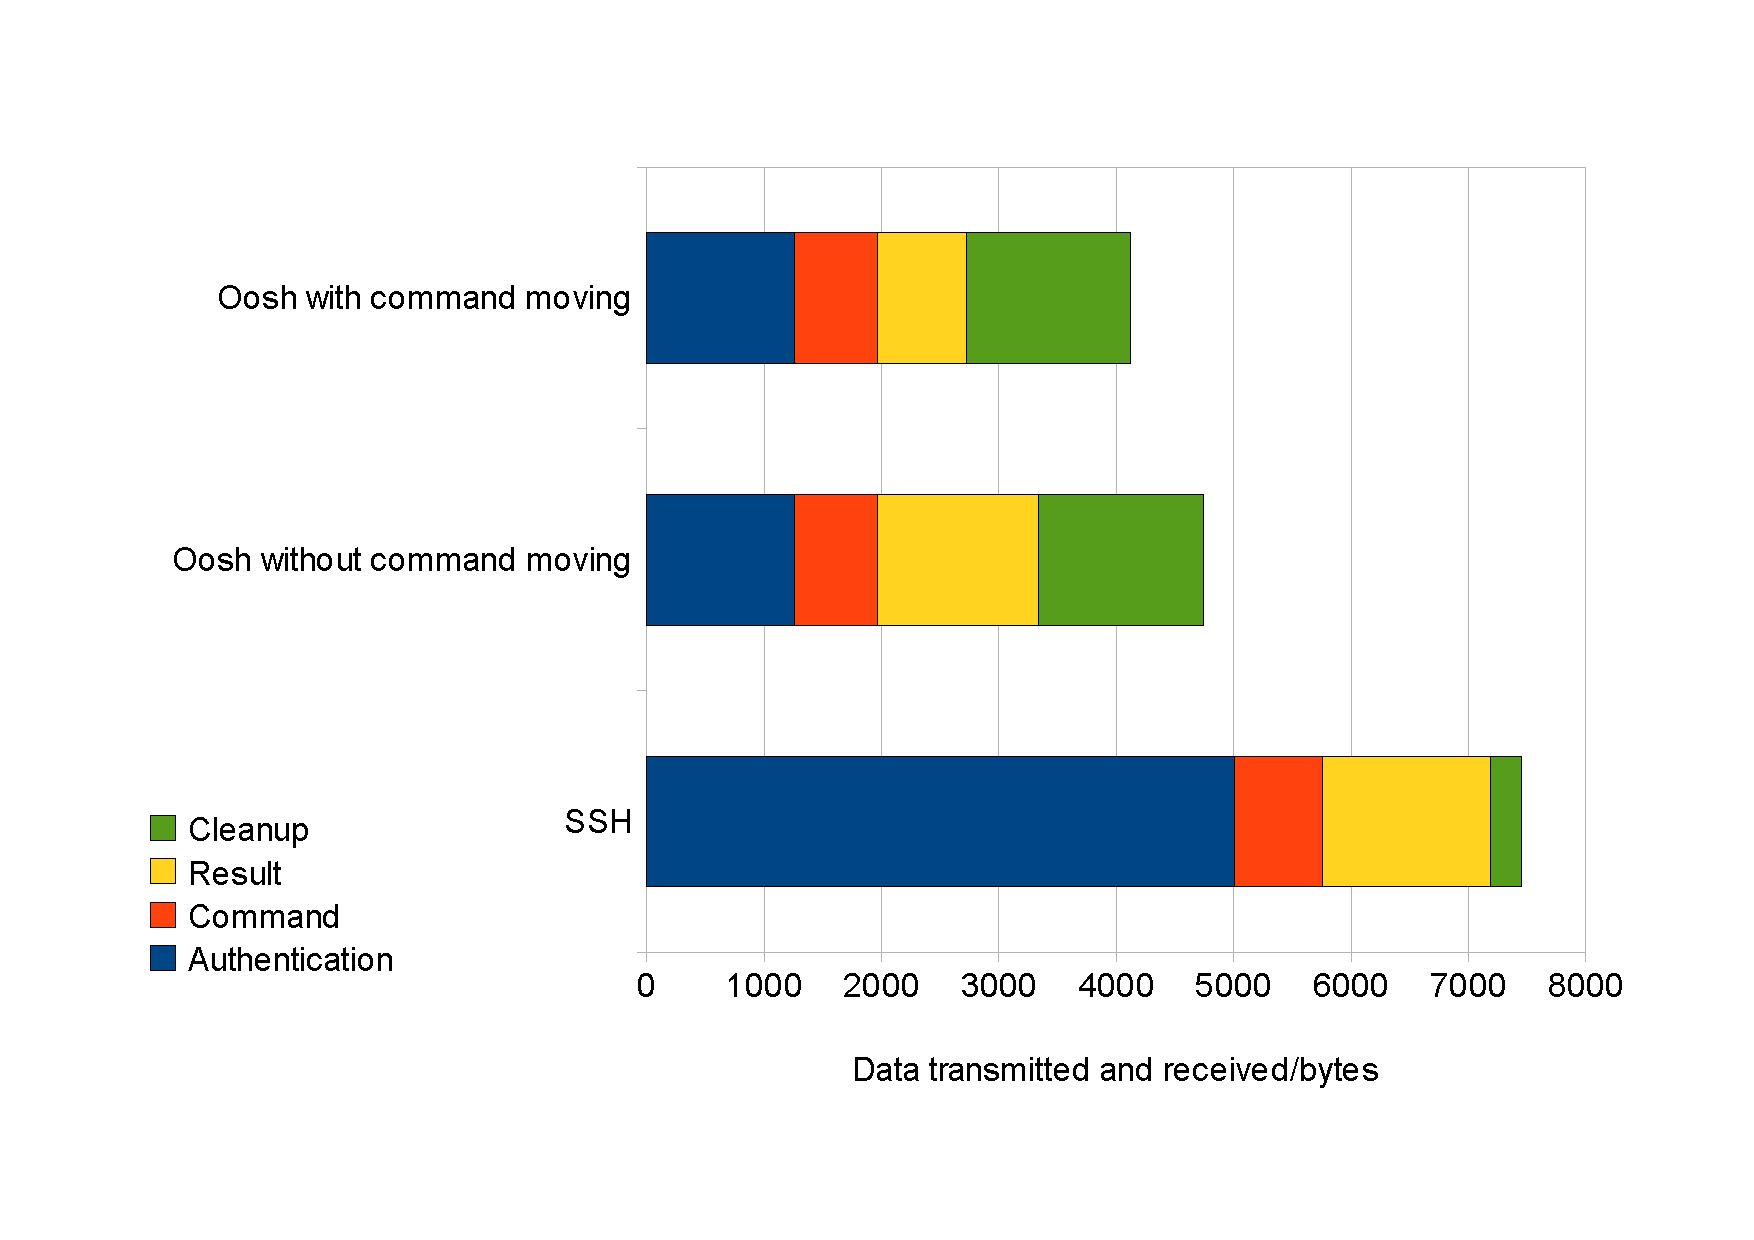
\includegraphics[scale=0.5]{network_graph.pdf}}
  \caption{Contrasting bandwidth usage between Bash with SSH and Oosh,
  and measuring the effect of command moving}
\label{networkgraph}
\end{figure}

Figure \ref{networkgraph} gives a side-by-side comparison of total
data sent for each of the three tests. The Bash with SSH test
demonstrates the additional complexity of the SSH authentication
protocol. This would be exacerbated if the user was interacting with a
larger number of servers. However this is a one-off cost and more
substantial commands running remotely would ensure the data returned
would be much larger than the authentication.

In the Oosh tests shown on the graph, there is noticeably less traffic
at the authentication stage due to the simpler protocol. Using the
command moving optimisation reduced the amount of data sent back from
1373 bytes (still slightly less than the 1436 bytes of SSH) to 698
bytes. However moving {\tt grep} to the remote system incurred a cost
(not shown on the graph) of 698 additional bytes for the second
command. Command moving in this example therefore only provides a very
modest bandwidth saving so savings are highly dependent on usage.

There is also a marked contrast between the 264 bytes required to
close the connection with SSH and the 1403 bytes required by
Oosh. This is partly due to Oosh requiring an explicit disconnection
message, but examining the traffic logs shows that Oosh initiates too
many TCP sessions. When the client initiates a session to the server
the server also starts a separate session to the client. This is
clearly wasteful because a single TCP connection supports duplex
communication. Much of the Oosh bandwidth is therefore wasted on TCP
setup and teardown. The 1403 bytes consisted of 20 packets, much
larger than SSH which only used 4. Consequently the average packet
size during Oosh cleanup was only 70 bytes. Since an empty TCP packet
is 66 bytes, clearly most of the 1403 bytes are superfluous.

Other optimisations become visible here as well. Oosh server commands
are sent as strings, and verbose messages reporting errors or lack
thereof are sent back as strings, even though successful execution
tends to be the most common outcome. The Oosh protocol is too chatty
and a shorter encoding for commands would also improve efficiency.

% bash with ssh:
% 24 packets 5005 authentication
% 6 packets 748 sending command
% 6 packets 1436 bytes sending data back (grep was local)
% 4 packets 264 bytes cleanup

% Oosh test without command moving:
% 18 packets, 1259 bytes (but 11 were runt packets) authentication
% 10 packets 708 bytes sending command
% 10 packets 1373 sending data back (grep local)
% 20 packets 1403 bytes cleanup

% Oosh with command moving:
% 18 packets, 1259 bytes authentication
% 10 packets 708 bytes sending first command
% 10 packets 698 bytes sending 2nd command
% 10 packets 752 bytes sending data back
% 20 packets 1403 cleanup

\section{Oosh Overheads}
I also conducted a series of benchmarks that measure the performance
overhead of using Oosh instead of standard tools.

\subsection{Overheads Due to Oosh Design Choices}
My first test compared running {\tt oosh\_ls} with {\tt ls} 6.12 from
GNU coreutils on a collection of directories with contents of varying
size. I generated these directories using the Bash command {\tt for x
  in \{1..n\}; do echo -n ``'' >\$x.txt; done} to ensure that all the
files were identical. Figure \ref{lsspeed} shows the performance
difference between the two.

\begin{figure}[h]
  \centering
  \setlength\fboxsep{0.5pt}
  \setlength\fboxrule{0.5pt}
  \fbox{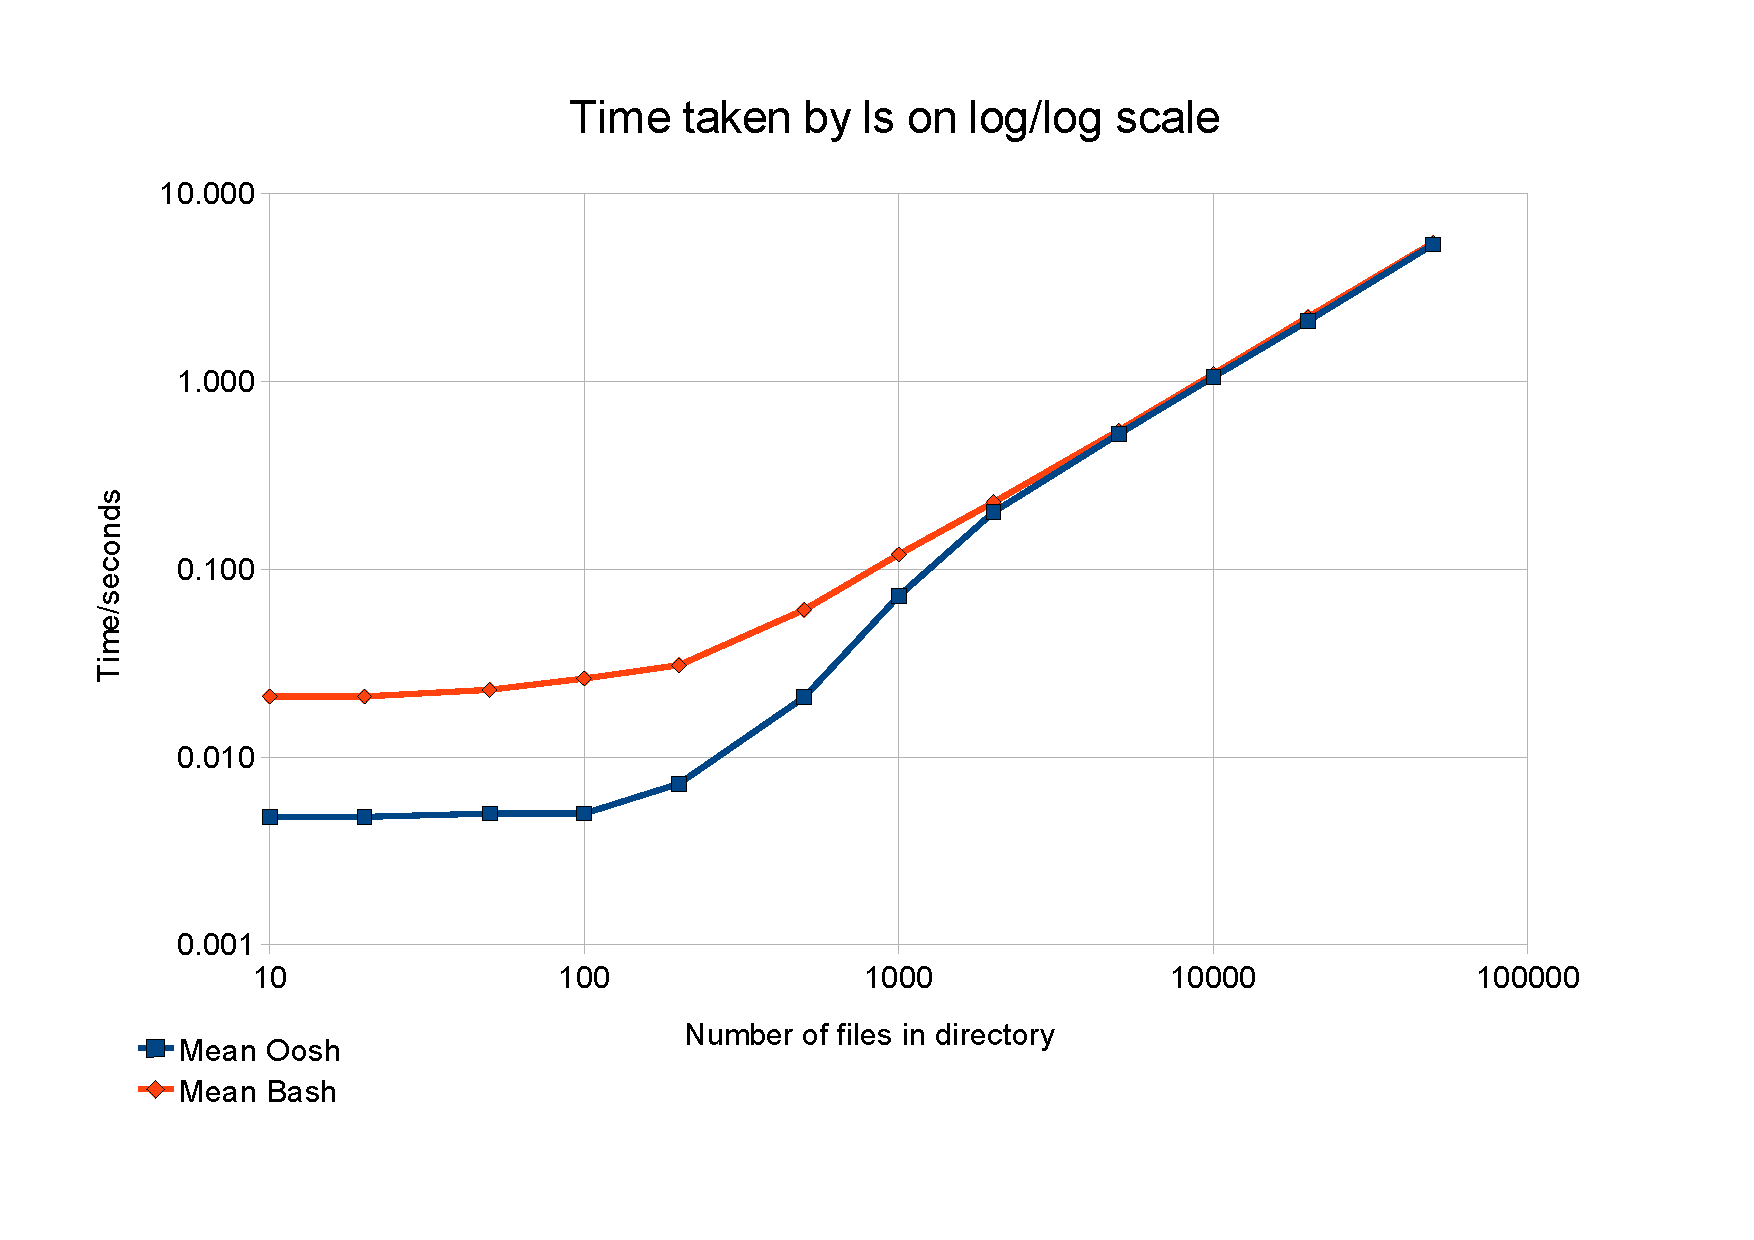
\includegraphics[scale=0.5]{ls_graph.pdf}}
  \caption{Contrasting performance between {\tt ls} from GNU Coreutils
    and {\tt oosh\_ls}}
\label{lsspeed}
\end{figure}

This graph demonstrates that there is very little performance overhead
when using Oosh for large datasets. At the lower end, Oosh commands
have a startup time of approximately 0.02 seconds which can be
attributed to the startup time of the Python interpreter. This
difference is below the level of human perception, although
pathological cases probably exist, such as an Oosh script with many
short lived processes. Humans cannot perceive delays of less than 0.1
seconds \cite{hci} so this delay is acceptable. Both {\tt ls} and {\tt
  oosh\_ls} can be seen to be scaling linearly with respect to the
number of files.

Testing the scaling of {\tt oosh\_ls} allowed me to analyse the costs
introduced by my data structure. If we consider a sample piece of output
from {\tt oosh\_ls} being run on the root directory, we obtain figure
\ref{lsroot}.

\begin{figure}[h]
\begin{Verbatim}[frame=single,framerule=0.2pt,framesep=5pt] 
{`Owner': `root', `Size': 4096, `Filename': `root'}
{`Owner': `root', `Size': 4096, `Filename': `media'}
{`Owner': `root', `Size': 0, `Filename': `.servers'}
{`Owner': `root', `Size': 0, `Filename': `.ux'}
{`Owner': `root', `Size': 3072, `Filename': `boot'}
{`Owner': `wrah2', `Size': 512, `Filename': `apps'}
{`Owner': `root', `Size': 12288, `Filename': `etc'}
{`Owner': `root', `Size': 4540, `Filename': `dev'}
{`Owner': `root', `Size': 0, `Filename': `proc'}
{`Owner': `root', `Size': 4096, `Filename': `opt'}
{`Owner': `root', `Size': 0, `Filename': `servers'}
{`Owner': `root', `Size': 36864, `Filename': `tmp'}
{`Owner': `root', `Size': 12288, `Filename': `authcon'}
{`Owner': `root', `Size': 12288, `Filename': `sbin'}
{`Owner': `root', `Size': 0, `Filename': `sys'}
{`Owner': `root', `Size': 12288, `Filename': `lib'}
{`Owner': `root', `Size': 4096, `Filename': `bin'}
{`Owner': `root', `Size': 4096, `Filename': `usr'}
{`Owner': `root', `Size': 4096, `Filename': `var'}
{`Owner': `wrah2', `Size': 512, `Filename': `ux'}
{`Owner': `root', `Size': 4096, `Filename': `srv'}
{`Owner': `root', `Size': 4096, `Filename': `mnt'}
{`Owner': `root', `Size': 16384, `Filename': `lost+found'}
{`Owner': `root', `Size': 12288, `Filename': `home'}
\end{Verbatim}
\caption{Output of {\tt oosh\_ls /} without pretty printing}
\label{lsroot}
\end{figure}

Data format efficiency was not a focus during the project, and as a
result the Oosh data structure contains some redundancies. One obvious
example is that of using curly brackets to mark the beginning and end
of lines when they are also separated by newline characters.  However
shell data is typically sent locally via local inter-process
communication which is sufficiently high bandwidth that we can afford
the additional overhead of Oosh structured data. To minimise data size
I could potentially use compression on each line, but as discussed in
section \ref{othermeasures}, CPU consumption is more of a concern with
Oosh so introducing compression would be unlikely to be a useful
optimisation.

\subsection{Latencies Introduced by Pretty Printing}
\label{prettyspeed}
As discussed in section \ref{prettyimpl}, my pretty printing algorithm
has complexity $O(C \log C + CL)$ in time, where $C$ is the number of
columns and $L$ the number of lines. Using the assumption that a
typical workload will have vastly more lines than columns in the
output, I measured the additional time taken for output to be shown to
the user if my pretty print algorithm is used.

\begin{figure}[h]
  \centering
  \setlength\fboxsep{2pt}
  \setlength\fboxrule{0.5pt}
  \fbox{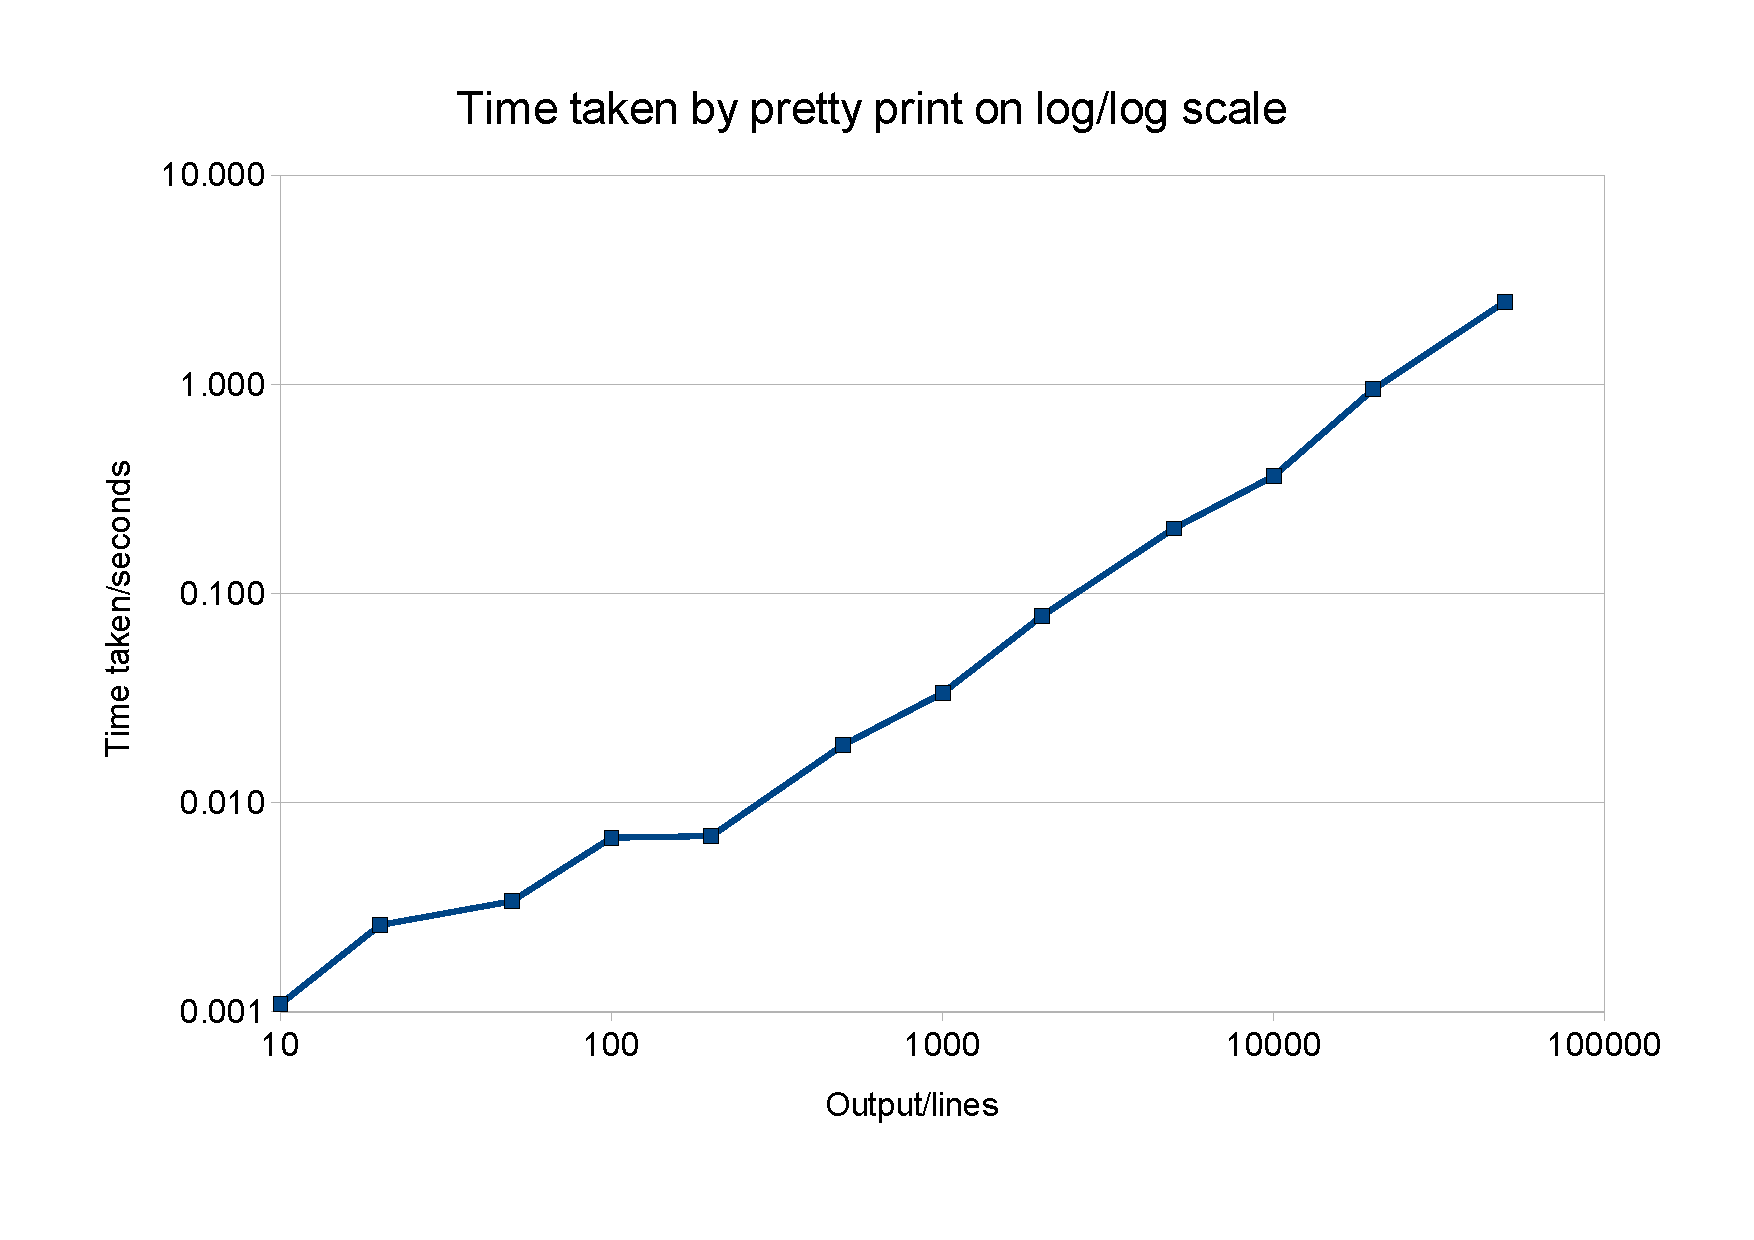
\includegraphics[scale=0.5]{print_graph.pdf}}
  \caption{Added latency due to running the pretty printing algorithm on
    Oosh output}
\end{figure}

This graph was produced using the same set of directories as in the
previous benchmark, and similarly using {\tt oosh\_ls}. I then
compared the time for the command to terminate with and without pretty
printing.

This graph conceals the fact that the pretty print algorithm requires
the full input before producing any output, whereas the simplistic
Bash-style approach of writing output asynchronously induces no
latency. The algorithm performs as expected, scaling roughly linearly
as the number of lines increases. Since printing 1000 lines introduces
only 33 milliseconds of delay (on top of the 93 milliseconds required
by the rest of the command execution), the performance of Oosh's
pretty print is completely acceptable for small or medium sized
quantities of data.

\subsection{Other Measures}
\label{othermeasures}

I also performed a few simpler measures of resource
utilisation. Whilst performing the pretty print benchmarks on the most
recent build of Oosh, I used the Linux resource monitor to measure
peak system usage. Memory usage peaked at 43 MiB, and CPU usage at 40\%
(on an Athlon 64 X2 6000 clocked at 3 GHz). By contrast, Bash did not
exceed 2 MiB of memory and 5\% CPU. The memory consumption is
acceptable on modern systems which tend to have at least 2 GiB of
memory. However CPU usage is rather high and since many experienced
shell users often have a number of shells open at once, this may
become a problem.

% what was evaluated?
% what were the results?
%   -- no of processes spawned
%   -- length of equivalent bash shells (can use old commands still!)
%   -- network data comparisons (fixed and variable cost increases measured)
%   -- performance
%     -- wall clock time
%     -- memory and CPU usage (never exceeded 43MiB memory during
%     benchmarks, or 40% CPU)
% testing/debugging
% comparing against requirements

\cleardoublepage
\chapter{Conclusions}

% aims again
% accomplishments -- likes, dislikes, results
% hindsight thoughts -- better approaches
% future prospects

\section{Overall Conclusions}

Developing Oosh demonstrated that it is possible to produce a more
effective shell metaphor provided that you only consider a limited
subset of shell functionality. The final product supports much of
standard Unix shell functionality plus a number of novel features. 

My structured data approach produced tangible benefits and making
networking part of the shell's built-ins produced new scope for
optimisations. Oosh is capable of dynamically determining whether it
is safe to move commands and transparently performing the move.

My graphing tools and data analysers offered particular clear benefits
from using structured data, and I would like to see these capabilities
incorporated into mainstream shells in the future.

As a standalone shell Oosh is not yet capable of replacing other
popular shells but as a proof of concept I believe it clearly displays
the potential of the Oosh design decisions.

\section{Potential Future Enhancements}
Throughout the project I found many features in common shells that are
widely used but were outside the scope of Oosh. However to use Oosh as
your primary shell would be very inconvenient without these.

One obvious enhancement would be pervasive use of the Oosh data
structure. There are a number of areas that would benefit from this.
One good example of this is the {\tt /sys} directory which holds
kernel generated hardware information. 

The precise format of the Oosh data structure was not chosen for
language independent manipulation. The Oosh data structure would
benefit from using a data format for which many tools exists, such as
XML or JSON (the format used currently is very nearly valid JSON).

Other missing luxuries include line continuations, regular
expressions, subshells (`backticks' in {\tt sh}) and tab completion. Tab
completion in Oosh could be substantially more powerful than that of
Bash, since commands can know column names.

I also did not take advantage of any of the optimising flags or
profiling tools within Python, so there probably is some potential for
improvement in Oosh's performance. My benchmarks showed that Oosh
performance was generally not much worse than that of Bash but large
workloads may well benefit from some careful optimisation.

% xml as data interchange format?

\cleardoublepage

%%%%%%%%%%%%%%%%%%%%%%%%%%%%%%%%%%%%%%%%%%%%%%%%%%%%%%%%%%%%%%%%%%%%%
% the bibliography

\addcontentsline{toc}{chapter}{Bibliography}
\begin{thebibliography}{11} % at most 11 citations

\bibitem{multics}
  Louis Pouzin
  \emph{Multics: The Origin of the Shell}
  \url{http://www.multicians.org/shell.html}

\bibitem{bourne}
  Tom Duff
  \emph{Rc -- A Shell for Plan 9 and UNIX systems}
  \url{http://doc.cat-v.org/plan\_9/4th\_edition/papers/rc}

\bibitem{fishdesign}
  Axel Liljencrantz
  \emph{Design Document}
  \url{http://fishshell.org/user\_doc/design.html}

\bibitem{gpl}
  Free Software Foundation
  \emph{The GNU General Public License}
  \url{http://www.gnu.org/licenses/gpl.html}

\bibitem{cc-by}
  Creative Commons
  \emph{Creative Commons Attribution 3.0 Unported License}
  \url{http://creativecommons.org/licenses/by/3.0/}

\bibitem{busybox}
  Denys Vlasenko
  \emph{BusyBox: The Swiss Army Knife of Embedded Linux}
  \url{http://www.busybox.net/about.html}

\bibitem{clifu}
  David Winterbottom
  \emph{commandlinefu.com is the place record those command-line gems that
  you return to again and again}
  \url{http://www.commandlinefu.com}

\bibitem{bashman}
  Free Software Foundation
  \emph{GNU bash manual}
  \url{http://www.gnu.org/software/bash/manual/}

\bibitem{hci}
  S.\ K.\ Card, T.\ P.\ Moran and A.\ Newell. 
  \emph{The Psychology of Human-Computer Interaction}

\bibitem{halstead}
  Halstead, Maurice H.\ 
  \emph{Elements of Software Science}
  Elsevier North-Holland, New York

\bibitem{ssh}
  Nicholas Rosasco and David Larochelle
  \emph{How and Why More Secure Technologies Succeed in Legacy
  Markets: Lessons from the Success of SSH}
  Department of Computer Science, University of Virginia   

\end{thebibliography}
\cleardoublepage

%%%%%%%%%%%%%%%%%%%%%%%%%%%%%%%%%%%%%%%%%%%%%%%%%%%%%%%%%%%%%%%%%%%%%
% the appendices
\appendix

\chapter{Project Proposal}
% makepdf.sh creates proposal_include.text

% use same formatting as proposal had in header
\parindent 0pt
\parskip 6pt
\include{proposal_include}

\chapter{Code Samples}

I have included the source code for {\tt oosh\_sort} as an example of
a command that understands the Oosh data format and acts
accordingly. I have also included the source code for the recursive
descent tree evaluator used within the shell itself.

\section{{\tt oosh\_sort.py}}

\begin{Verbatim}[commandchars=\\\{\}]
\PY{k+kn}{import} \PY{n+nn}{sys}
\PY{k+kn}{import} \PY{n+nn}{operator}
\PY{k+kn}{import} \PY{n+nn}{oosh}
\PY{k+kn}{from} \PY{n+nn}{oosh} \PY{k+kn}{import} \PY{n}{OoshError}

\PY{n}{args} \PY{o}{=} \PY{n}{sys}\PY{o}{.}\PY{n}{argv}\PY{p}{[}\PY{l+m+mi}{1}\PY{p}{:}\PY{p}{]}
\PY{k}{if} \PY{n+nb}{len}\PY{p}{(}\PY{n}{args}\PY{p}{)} \PY{o}{<} \PY{l+m+mi}{1}\PY{p}{:}
    \PY{k}{print}\PY{p}{(}\PY{l+s}{"}\PY{l+s}{Usage: oosh\PYZus{}sort columnname}\PY{l+s}{"}\PY{p}{)}
    \PY{n}{sys}\PY{o}{.}\PY{n}{exit}\PY{p}{(}\PY{l+m+mi}{1}\PY{p}{)}

\PY{n}{sort\PYZus{}on} \PY{o}{=} \PY{n}{args}\PY{p}{[}\PY{l+m+mi}{0}\PY{p}{]}
\PY{n}{pipein} \PY{o}{=} \PY{n}{sys}\PY{o}{.}\PY{n}{stdin}\PY{o}{.}\PY{n}{read}\PY{p}{(}\PY{p}{)}\PY{o}{.}\PY{n}{splitlines}\PY{p}{(}\PY{p}{)}
\PY{n}{lines} \PY{o}{=} \PY{n}{oosh}\PY{o}{.}\PY{n}{get\PYZus{}from\PYZus{}pipe}\PY{p}{(}\PY{n}{pipein}\PY{p}{)}
\PY{c}{# check we are sorting on a valid column}
\PY{k}{if} \PY{n+nb}{len}\PY{p}{(}\PY{n}{lines}\PY{p}{)} \PY{o}{>} \PY{l+m+mi}{0} \PY{o+ow}{and} \PY{n}{sort\PYZus{}on} \PY{o+ow}{not} \PY{o+ow}{in} \PY{n}{lines}\PY{p}{[}\PY{l+m+mi}{0}\PY{p}{]}\PY{o}{.}\PY{n}{keys}\PY{p}{(}\PY{p}{)}\PY{p}{:}
    \PY{k}{print}\PY{p}{(}\PY{n}{sort\PYZus{}on}\PY{p}{,}\PY{l+s}{"}\PY{l+s}{is not a valid column name}\PY{l+s}{"}\PY{p}{)}
    \PY{n}{sys}\PY{o}{.}\PY{n}{exit}\PY{p}{(}\PY{l+m+mi}{1}\PY{p}{)}  

\PY{c}{# treat data numerically if possible, it comes in as a string}
\PY{c}{# preferring whole numbers if possible}
\PY{n}{is\PYZus{}numeric} \PY{o}{=} \PY{n+nb+bp}{True}
\PY{k}{for} \PY{n}{line} \PY{o+ow}{in} \PY{n}{lines}\PY{p}{:}
    \PY{k}{try}\PY{p}{:}
        \PY{n}{line}\PY{p}{[}\PY{n}{sort\PYZus{}on}\PY{p}{]} \PY{o}{=} \PY{n+nb}{int}\PY{p}{(}\PY{n}{line}\PY{p}{[}\PY{n}{sort\PYZus{}on}\PY{p}{]}\PY{p}{)}
    \PY{k}{except} \PY{n+ne}{ValueError}\PY{p}{:}
        \PY{k}{try}\PY{p}{:}
            \PY{n}{line}\PY{p}{[}\PY{n}{sort\PYZus{}on}\PY{p}{]} \PY{o}{=} \PY{n+nb}{float}\PY{p}{(}\PY{n}{line}\PY{p}{[}\PY{n}{sort\PYZus{}on}\PY{p}{]}\PY{p}{)}
        \PY{k}{except} \PY{n+ne}{ValueError}\PY{p}{:}
            \PY{n}{is\PYZus{}numeric} \PY{o}{=} \PY{n+nb+bp}{False}
            \PY{k}{break}
\PY{c}{# if we have mixed data, we may have converted to float/int, so revert}
\PY{k}{if} \PY{o+ow}{not} \PY{n}{is\PYZus{}numeric}\PY{p}{:}
    \PY{k}{for} \PY{n}{line} \PY{o+ow}{in} \PY{n}{lines}\PY{p}{:}
        \PY{n}{line}\PY{p}{[}\PY{n}{sort\PYZus{}on}\PY{p}{]} \PY{o}{=} \PY{n+nb}{str}\PY{p}{(}\PY{n}{line}\PY{p}{[}\PY{n}{sort\PYZus{}on}\PY{p}{]}\PY{p}{)}

\PY{n}{lines}\PY{o}{.}\PY{n}{sort}\PY{p}{(}\PY{n}{key}\PY{o}{=}\PY{n}{operator}\PY{o}{.}\PY{n}{itemgetter}\PY{p}{(}\PY{n}{sort\PYZus{}on}\PY{p}{)}\PY{p}{)}
\PY{k}{for} \PY{n}{dic} \PY{o+ow}{in} \PY{n}{lines}\PY{p}{:}
    \PY{n}{sys}\PY{o}{.}\PY{n}{stdout}\PY{o}{.}\PY{n}{write}\PY{p}{(}\PY{n}{dic}\PY{o}{.}\PY{n}{\PYZus{}\PYZus{}repr\PYZus{}\PYZus{}}\PY{p}{(}\PY{p}{)} \PY{o}{+} \PY{l+s}{`}\PY{l+s+se}{\PYZbs{}n}\PY{l+s}{'}\PY{p}{)}
\end{Verbatim}

\section{Tree Evaluator}
\begin{Verbatim}[commandchars=\\\{\}]
\PY{k}{def} \PY{n+nf}{eval\PYZus{}tree}\PY{p}{(}\PY{n+nb+bp}{self}\PY{p}{,} \PY{n}{ast}\PY{p}{,} \PY{n}{pipe\PYZus{}pointer}\PY{p}{)}\PY{p}{:}
    \PY{c}{# recurse down tree, starting processes and passing pointers}
    \PY{c}{# of pipes created as appopriate.}

    \PY{c}{# returns a tuple (stdout\PYZus{}pipe\PYZus{}pointer, return\PYZus{}code)}
        
    \PY{k}{if} \PY{n}{ast} \PY{o+ow}{is} \PY{n+nb+bp}{None}\PY{p}{:}
        \PY{k}{print}\PY{p}{(}\PY{l+s}{`}\PY{l+s}{Evaluated empty tree}\PY{l+s}{'}\PY{p}{)}
        \PY{k}{return} \PY{p}{(}\PY{n}{PipePointer}\PY{p}{(}\PY{p}{)}\PY{p}{,} \PY{l+m+mi}{0}\PY{p}{)}

    \PY{k}{if} \PY{n}{ast}\PY{p}{[}\PY{l+m+mi}{0}\PY{p}{]} \PY{o}{==} \PY{l+s}{`}\PY{l+s}{sequence}\PY{l+s}{'}\PY{p}{:}
        \PY{p}{(}\PY{n}{stdout}\PY{p}{,} \PY{n}{returncode}\PY{p}{)} \PY{o}{=} \PY{n+nb+bp}{self}\PY{o}{.}\PY{n}{eval\PYZus{}tree}\PY{p}{(}\PY{n}{ast}\PY{p}{[}\PY{l+m+mi}{1}\PY{p}{]}\PY{p}{,} \PY{n}{PipePointer}\PY{p}{(}\PY{p}{)}\PY{p}{)}
        \PY{n+nb+bp}{self}\PY{o}{.}\PY{n}{output\PYZus{}for\PYZus{}user}\PY{o}{.}\PY{n}{append}\PY{p}{(}\PY{n}{stdout}\PY{p}{)}
        \PY{k}{return} \PY{n+nb+bp}{self}\PY{o}{.}\PY{n}{eval\PYZus{}tree}\PY{p}{(}\PY{n}{ast}\PY{p}{[}\PY{l+m+mi}{2}\PY{p}{]}\PY{p}{,} \PY{n}{PipePointer}\PY{p}{(}\PY{p}{)}\PY{p}{)}

    \PY{k}{elif} \PY{n}{ast}\PY{p}{[}\PY{l+m+mi}{0}\PY{p}{]} \PY{o}{==} \PY{l+s}{`}\PY{l+s}{savepipe}\PY{l+s}{'}\PY{p}{:}
        \PY{p}{(}\PY{n}{pipe\PYZus{}out}\PY{p}{,} \PY{n}{return\PYZus{}code}\PY{p}{)} \PY{o}{=} \PY{n+nb+bp}{self}\PY{o}{.}\PY{n}{eval\PYZus{}tree}\PY{p}{(}\PY{n}{ast}\PY{p}{[}\PY{l+m+mi}{1}\PY{p}{]}\PY{p}{,} \PY{n}{PipePointer}\PY{p}{(}\PY{p}{)}\PY{p}{)}
        \PY{n}{pipe\PYZus{}number} \PY{o}{=} \PY{n}{ast}\PY{p}{[}\PY{l+m+mi}{2}\PY{p}{]}\PY{p}{[}\PY{l+m+mi}{1}\PY{p}{:}\PY{p}{]}
        \PY{n+nb+bp}{self}\PY{o}{.}\PY{n}{saved\PYZus{}pipe\PYZus{}data}\PY{p}{[}\PY{n}{pipe\PYZus{}number}\PY{p}{]} \PY{o}{=} \PY{n}{pipe\PYZus{}out}\PY{o}{.}\PY{n}{read}\PY{p}{(}\PY{p}{)}
        \PY{k}{return} \PY{p}{(}\PY{n}{PipePointer}\PY{p}{(}\PY{p}{)}\PY{p}{,} \PY{n}{return\PYZus{}code}\PY{p}{)}

    \PY{k}{elif} \PY{n}{ast}\PY{p}{[}\PY{l+m+mi}{0}\PY{p}{]} \PY{o}{==} \PY{l+s}{`}\PY{l+s}{for}\PY{l+s}{'}\PY{p}{:}
        \PY{n}{old\PYZus{}variables} \PY{o}{=} \PY{n+nb+bp}{self}\PY{o}{.}\PY{n}{variables}\PY{o}{.}\PY{n}{copy}\PY{p}{(}\PY{p}{)}
        \PY{k}{for} \PY{n}{value} \PY{o+ow}{in} \PY{n+nb+bp}{self}\PY{o}{.}\PY{n}{flatten\PYZus{}tree}\PY{p}{(}\PY{n}{ast}\PY{p}{[}\PY{l+m+mi}{2}\PY{p}{]}\PY{p}{)}\PY{p}{:}
            \PY{n+nb+bp}{self}\PY{o}{.}\PY{n}{variables}\PY{p}{[}\PY{n}{ast}\PY{p}{[}\PY{l+m+mi}{1}\PY{p}{]}\PY{p}{]} \PY{o}{=} \PY{n}{value}
            \PY{p}{(}\PY{n}{stdout}\PY{p}{,} \PY{n}{return\PYZus{}code}\PY{p}{)} \PY{o}{=} \PY{n+nb+bp}{self}\PY{o}{.}\PY{n}{eval\PYZus{}tree}\PY{p}{(}\PY{n}{ast}\PY{p}{[}\PY{l+m+mi}{3}\PY{p}{]}\PY{p}{,} \PY{n}{PipePointer}\PY{p}{(}\PY{p}{)}\PY{p}{)}
            \PY{n+nb+bp}{self}\PY{o}{.}\PY{n}{output\PYZus{}for\PYZus{}user}\PY{o}{.}\PY{n}{append}\PY{p}{(}\PY{n}{stdout}\PY{p}{)}
        \PY{n+nb+bp}{self}\PY{o}{.}\PY{n}{variables} \PY{o}{=} \PY{n}{old\PYZus{}variables}
        \PY{k}{return} \PY{p}{(}\PY{n}{PipePointer}\PY{p}{(}\PY{p}{)}\PY{p}{,} \PY{n}{return\PYZus{}code}\PY{p}{)}

    \PY{k}{elif} \PY{n}{ast}\PY{p}{[}\PY{l+m+mi}{0}\PY{p}{]} \PY{o}{==} \PY{l+s}{`}\PY{l+s}{while}\PY{l+s}{'}\PY{p}{:}
        \PY{k}{while} \PY{n}{return\PYZus{}code} \PY{o}{==} \PY{l+m+mi}{0}\PY{p}{:}
            \PY{p}{(}\PY{n}{dont\PYZus{}care}\PY{p}{,} \PY{n}{return\PYZus{}code}\PY{p}{)} \PY{o}{=} \PY{n+nb+bp}{self}\PY{o}{.}\PY{n}{eval\PYZus{}tree}\PY{p}{(}\PY{n}{ast}\PY{p}{[}\PY{l+m+mi}{1}\PY{p}{]}\PY{p}{,} \PY{n}{PipePointer}\PY{p}{(}\PY{p}{)}\PY{p}{)}
            \PY{p}{(}\PY{n}{stdout}\PY{p}{,} \PY{n}{final\PYZus{}return\PYZus{}code}\PY{p}{)} \PY{o}{=} \PY{n+nb+bp}{self}\PY{o}{.}\PY{n}{eval\PYZus{}tree}\PY{p}{(}\PY{n}{ast}\PY{p}{[}\PY{l+m+mi}{2}\PY{p}{]}\PY{p}{,} \PY{n}{PipePointer}\PY{p}{(}\PY{p}{)}\PY{p}{)}
            \PY{n+nb+bp}{self}\PY{o}{.}\PY{n}{output\PYZus{}for\PYZus{}user}\PY{o}{.}\PY{n}{append}\PY{p}{(}\PY{n}{stdout}\PY{p}{)}
        \PY{k}{return} \PY{p}{(}\PY{n}{PipePointer}\PY{p}{(}\PY{p}{)}\PY{p}{,} \PY{n}{final\PYZus{}return\PYZus{}code}\PY{p}{)}

    \PY{k}{elif} \PY{n}{ast}\PY{p}{[}\PY{l+m+mi}{0}\PY{p}{]} \PY{o}{==} \PY{l+s}{`}\PY{l+s}{if}\PY{l+s}{'}\PY{p}{:}
        \PY{p}{(}\PY{n}{stdout}\PY{p}{,} \PY{n}{return\PYZus{}code}\PY{p}{)} \PY{o}{=} \PY{n+nb+bp}{self}\PY{o}{.}\PY{n}{eval\PYZus{}tree}\PY{p}{(}\PY{n}{ast}\PY{p}{[}\PY{l+m+mi}{1}\PY{p}{]}\PY{p}{,} \PY{n}{PipePointer}\PY{p}{(}\PY{p}{)}\PY{p}{)}
        \PY{k}{if} \PY{n}{return\PYZus{}code} \PY{o}{==} \PY{l+m+mi}{0}\PY{p}{:} \PY{c}{# 0 is true for shells}
            \PY{k}{return} \PY{n+nb+bp}{self}\PY{o}{.}\PY{n}{eval\PYZus{}tree}\PY{p}{(}\PY{n}{ast}\PY{p}{[}\PY{l+m+mi}{2}\PY{p}{]}\PY{p}{,} \PY{n}{PipePointer}\PY{p}{(}\PY{p}{)}\PY{p}{)}
        \PY{k}{else}\PY{p}{:}
            \PY{k}{return} \PY{p}{(}\PY{n}{PipePointer}\PY{p}{(}\PY{p}{)}\PY{p}{,} \PY{l+m+mi}{0}\PY{p}{)}

    \PY{k}{elif} \PY{n}{ast}\PY{p}{[}\PY{l+m+mi}{0}\PY{p}{]} \PY{o}{==} \PY{l+s}{`}\PY{l+s}{if-else}\PY{l+s}{'}\PY{p}{:}
        \PY{p}{(}\PY{n}{stdout}\PY{p}{,} \PY{n}{return\PYZus{}code}\PY{p}{)} \PY{o}{=} \PY{n+nb+bp}{self}\PY{o}{.}\PY{n}{eval\PYZus{}tree}\PY{p}{(}\PY{n}{ast}\PY{p}{[}\PY{l+m+mi}{1}\PY{p}{]}\PY{p}{,} \PY{n}{PipePointer}\PY{p}{(}\PY{p}{)}\PY{p}{)}
        \PY{k}{if} \PY{n}{return\PYZus{}code} \PY{o}{==} \PY{l+m+mi}{0}\PY{p}{:}
            \PY{k}{return} \PY{n+nb+bp}{self}\PY{o}{.}\PY{n}{eval\PYZus{}tree}\PY{p}{(}\PY{n}{ast}\PY{p}{[}\PY{l+m+mi}{2}\PY{p}{]}\PY{p}{,} \PY{n}{PipePointer}\PY{p}{(}\PY{p}{)}\PY{p}{)}
        \PY{k}{else}\PY{p}{:}
            \PY{k}{return} \PY{n+nb+bp}{self}\PY{o}{.}\PY{n}{eval\PYZus{}tree}\PY{p}{(}\PY{n}{ast}\PY{p}{[}\PY{l+m+mi}{3}\PY{p}{]}\PY{p}{,} \PY{n}{PipePointer}\PY{p}{(}\PY{p}{)}\PY{p}{)}

    \PY{k}{elif} \PY{n}{ast}\PY{p}{[}\PY{l+m+mi}{0}\PY{p}{]} \PY{o}{==} \PY{l+s}{`}\PY{l+s}{assign}\PY{l+s}{'}\PY{p}{:}
        \PY{n+nb+bp}{self}\PY{o}{.}\PY{n}{variables}\PY{p}{[}\PY{n}{ast}\PY{p}{[}\PY{l+m+mi}{1}\PY{p}{]}\PY{p}{]} \PY{o}{=} \PY{n+nb+bp}{self}\PY{o}{.}\PY{n}{flatten\PYZus{}tree}\PY{p}{(}\PY{n}{ast}\PY{p}{[}\PY{l+m+mi}{2}\PY{p}{]}\PY{p}{)}\PY{p}{[}\PY{l+m+mi}{0}\PY{p}{]}
        \PY{k}{return} \PY{p}{(}\PY{n}{PipePointer}\PY{p}{(}\PY{p}{)}\PY{p}{,} \PY{l+m+mi}{0}\PY{p}{)}

    \PY{k}{elif} \PY{n}{ast}\PY{p}{[}\PY{l+m+mi}{0}\PY{p}{]} \PY{o}{==} \PY{l+s}{`}\PY{l+s}{derefpipe}\PY{l+s}{'}\PY{p}{:}
        \PY{c}{# create a process to give us a stdout to pass}
        \PY{c}{# to whatever is next in the pipeline}
        \PY{n}{old\PYZus{}pipe\PYZus{}name} \PY{o}{=} \PY{n}{ast}\PY{p}{[}\PY{l+m+mi}{1}\PY{p}{]}\PY{p}{[}\PY{l+m+mi}{1}\PY{p}{:}\PY{p}{]} \PY{c}{# e.g. |2}
        \PY{k}{try}\PY{p}{:}
            \PY{n}{old\PYZus{}pipe\PYZus{}data} \PY{o}{=} \PY{n+nb+bp}{self}\PY{o}{.}\PY{n}{saved\PYZus{}pipe\PYZus{}data}\PY{p}{[}\PY{n}{old\PYZus{}pipe\PYZus{}name}\PY{p}{]}
            \PY{n}{old\PYZus{}pipe\PYZus{}pointer} \PY{o}{=} \PY{n+nb+bp}{self}\PY{o}{.}\PY{n}{pipe\PYZus{}from\PYZus{}data}\PY{p}{(}\PY{n}{old\PYZus{}pipe\PYZus{}data}\PY{p}{)}
            \PY{k}{return} \PY{n+nb+bp}{self}\PY{o}{.}\PY{n}{eval\PYZus{}tree}\PY{p}{(}\PY{n}{ast}\PY{p}{[}\PY{l+m+mi}{2}\PY{p}{]}\PY{p}{,} \PY{n}{PipePointer}\PY{p}{(}\PY{n}{old\PYZus{}pipe\PYZus{}pointer}\PY{p}{)}\PY{p}{)}
        \PY{k}{except} \PY{n+ne}{KeyError}\PY{p}{:}
            \PY{k}{raise} \PY{n}{OoshError}\PY{p}{(}\PY{l+s}{"}\PY{l+s}{You have not saved a pipe numbered }\PY{l+s}{"} \PY{o}{+}
                            \PY{n}{old\PYZus{}pipe\PYZus{}name}\PY{p}{)}

    \PY{k}{elif} \PY{n}{ast}\PY{p}{[}\PY{l+m+mi}{0}\PY{p}{]} \PY{o}{==} \PY{l+s}{`}\PY{l+s}{simplecommand}\PY{l+s}{'}\PY{p}{:}
        \PY{n}{command} \PY{o}{=} \PY{n+nb+bp}{self}\PY{o}{.}\PY{n}{flatten\PYZus{}tree}\PY{p}{(}\PY{n}{ast}\PY{p}{[}\PY{l+m+mi}{1}\PY{p}{]}\PY{p}{)}
        \PY{k}{return} \PY{n+nb+bp}{self}\PY{o}{.}\PY{n}{shell\PYZus{}command}\PY{p}{(}\PY{n}{command}\PY{p}{,} \PY{n}{pipe\PYZus{}pointer}\PY{p}{)}

    \PY{k}{elif} \PY{n}{ast}\PY{p}{[}\PY{l+m+mi}{0}\PY{p}{]} \PY{o}{==} \PY{l+s}{`}\PY{l+s}{derefmultipipe}\PY{l+s}{'}\PY{p}{:}
        \PY{n}{pipe\PYZus{}names} \PY{o}{=} \PY{n}{ast}\PY{p}{[}\PY{l+m+mi}{1}\PY{p}{]}\PY{p}{[}\PY{l+m+mi}{1}\PY{p}{:}\PY{p}{]}\PY{o}{.}\PY{n}{split}\PY{p}{(}\PY{l+s}{`}\PY{l+s}{+}\PY{l+s}{'}\PY{p}{)}

        \PY{n}{first\PYZus{}pipe\PYZus{}data} \PY{o}{=} \PY{n+nb+bp}{self}\PY{o}{.}\PY{n}{saved\PYZus{}pipe\PYZus{}data}\PY{p}{[}\PY{n}{pipe\PYZus{}names}\PY{p}{[}\PY{l+m+mi}{0}\PY{p}{]}\PY{p}{]}
        \PY{n}{first\PYZus{}pipe\PYZus{}pointer} \PY{o}{=} \PY{n+nb+bp}{self}\PY{o}{.}\PY{n}{pipe\PYZus{}from\PYZus{}data}\PY{p}{(}\PY{n}{first\PYZus{}pipe\PYZus{}data}\PY{p}{)}

        \PY{n}{second\PYZus{}pipe\PYZus{}data} \PY{o}{=} \PY{n+nb+bp}{self}\PY{o}{.}\PY{n}{saved\PYZus{}pipe\PYZus{}data}\PY{p}{[}\PY{n}{pipe\PYZus{}names}\PY{p}{[}\PY{l+m+mi}{1}\PY{p}{]}\PY{p}{]}
        \PY{n}{second\PYZus{}pipe\PYZus{}pointer} \PY{o}{=} \PY{n+nb+bp}{self}\PY{o}{.}\PY{n}{pipe\PYZus{}from\PYZus{}data}\PY{p}{(}\PY{n}{second\PYZus{}pipe\PYZus{}data}\PY{p}{)}

        \PY{c}{# we call command, appending argument of second pipe}
        \PY{n}{command} \PY{o}{=} \PY{n+nb+bp}{self}\PY{o}{.}\PY{n}{flatten\PYZus{}tree}\PY{p}{(}\PY{n}{ast}\PY{p}{[}\PY{l+m+mi}{2}\PY{p}{]}\PY{p}{[}\PY{l+m+mi}{1}\PY{p}{]}\PY{p}{)}
        \PY{n}{command}\PY{o}{.}\PY{n}{append}\PY{p}{(}\PY{n+nb}{str}\PY{p}{(}\PY{n}{second\PYZus{}pipe\PYZus{}pointer}\PY{o}{.}\PY{n}{fileno}\PY{p}{(}\PY{p}{)}\PY{p}{)}\PY{p}{)}

        \PY{c}{# check user hasn't tried to run this remotely}
        \PY{k}{if} \PY{n+nb+bp}{self}\PY{o}{.}\PY{n}{specifies\PYZus{}location}\PY{p}{(}\PY{n}{command}\PY{p}{[}\PY{l+m+mi}{0}\PY{p}{]}\PY{p}{)}\PY{p}{:}
            \PY{k}{raise} \PY{n}{OoshError}\PY{p}{(}\PY{l+s}{"}\PY{l+s}{Cannot run multipipe commands remotely}\PY{l+s}{"}\PY{p}{)}
            
        \PY{k}{return} \PY{n+nb+bp}{self}\PY{o}{.}\PY{n}{shell\PYZus{}command}\PY{p}{(}\PY{n}{command}\PY{p}{,} \PY{n}{PipePointer}\PY{p}{(}\PY{n}{first\PYZus{}pipe\PYZus{}pointer}\PY{p}{)}\PY{p}{)}

    \PY{k}{elif} \PY{n}{ast}\PY{p}{[}\PY{l+m+mi}{0}\PY{p}{]} \PY{o}{==} \PY{l+s}{`}\PY{l+s}{pipedcommand}\PY{l+s}{'}\PY{p}{:}
        \PY{p}{(}\PY{n}{stdout}\PY{p}{,} \PY{n}{return\PYZus{}code}\PY{p}{)} \PY{o}{=} \PY{n+nb+bp}{self}\PY{o}{.}\PY{n}{eval\PYZus{}tree}\PY{p}{(}\PY{n}{ast}\PY{p}{[}\PY{l+m+mi}{1}\PY{p}{]}\PY{p}{,} \PY{n}{pipe\PYZus{}pointer}\PY{p}{)}
        \PY{k}{return} \PY{n+nb+bp}{self}\PY{o}{.}\PY{n}{eval\PYZus{}tree}\PY{p}{(}\PY{n}{ast}\PY{p}{[}\PY{l+m+mi}{2}\PY{p}{]}\PY{p}{,} \PY{n}{stdout}\PY{p}{)}

    \PY{k}{elif} \PY{n}{ast}\PY{p}{[}\PY{l+m+mi}{0}\PY{p}{]} \PY{o+ow}{is} \PY{n+nb+bp}{None}\PY{p}{:} \PY{c}{# occurs with trailing ;}
        \PY{k}{pass}

    \PY{k}{else}\PY{p}{:}
        \PY{k}{raise} \PY{n}{OoshError}\PY{p}{(}\PY{l+s}{"}\PY{l+s}{Unknown tree }\PY{l+s}{"} \PY{o}{+} \PY{n+nb}{str}\PY{p}{(}\PY{n}{ast}\PY{p}{)}\PY{p}{)}
\end{Verbatim}

\end{document}
